%\chapter{Control System for Complete Complex Autonomous Systems: Hubo-Ach}\label{sec:hubo-ach}
%\chapter{Thesis: Hubo-Ach - A Control System for Complete Complex Autonomous Systems}\label{sec:hubo-ach}
\chapter{Hubo-Ach: Control System for Complete Complex Autonomous Systems}\label{sec:hubo-ach}

%% Hubo-Ach Inspiration
\section{Overview}

%% Hubo-Ach explanation
%% workign wth ros and other software that exists, why in C



%\section{Hubo-Ach: Linux on Hubo}

The Hubo2+ is a $1.3\meter$ tall, $42 \kilo\gram$ full-size humanoid
robot, produced by the Korean Advanced Institute of Science and
Technology (KAIST) and spinoff company Rainbow Inc. \cite{1573587}.
It has 38 DOF: six per arm and leg, five per hand, three in the neck,
and one in the waist.  Sensors include three-axis force-torque sensors
in the wrists and ankles, accelerometers in the feet, and an inertial
measurement unit (IMU).  The sensors and embedded motor controllers
are connected via a Controller Area Network to a pair of Intel Atom
PC104+ PCs.

% \begin{figure*}[thpb]
%   \centering
% 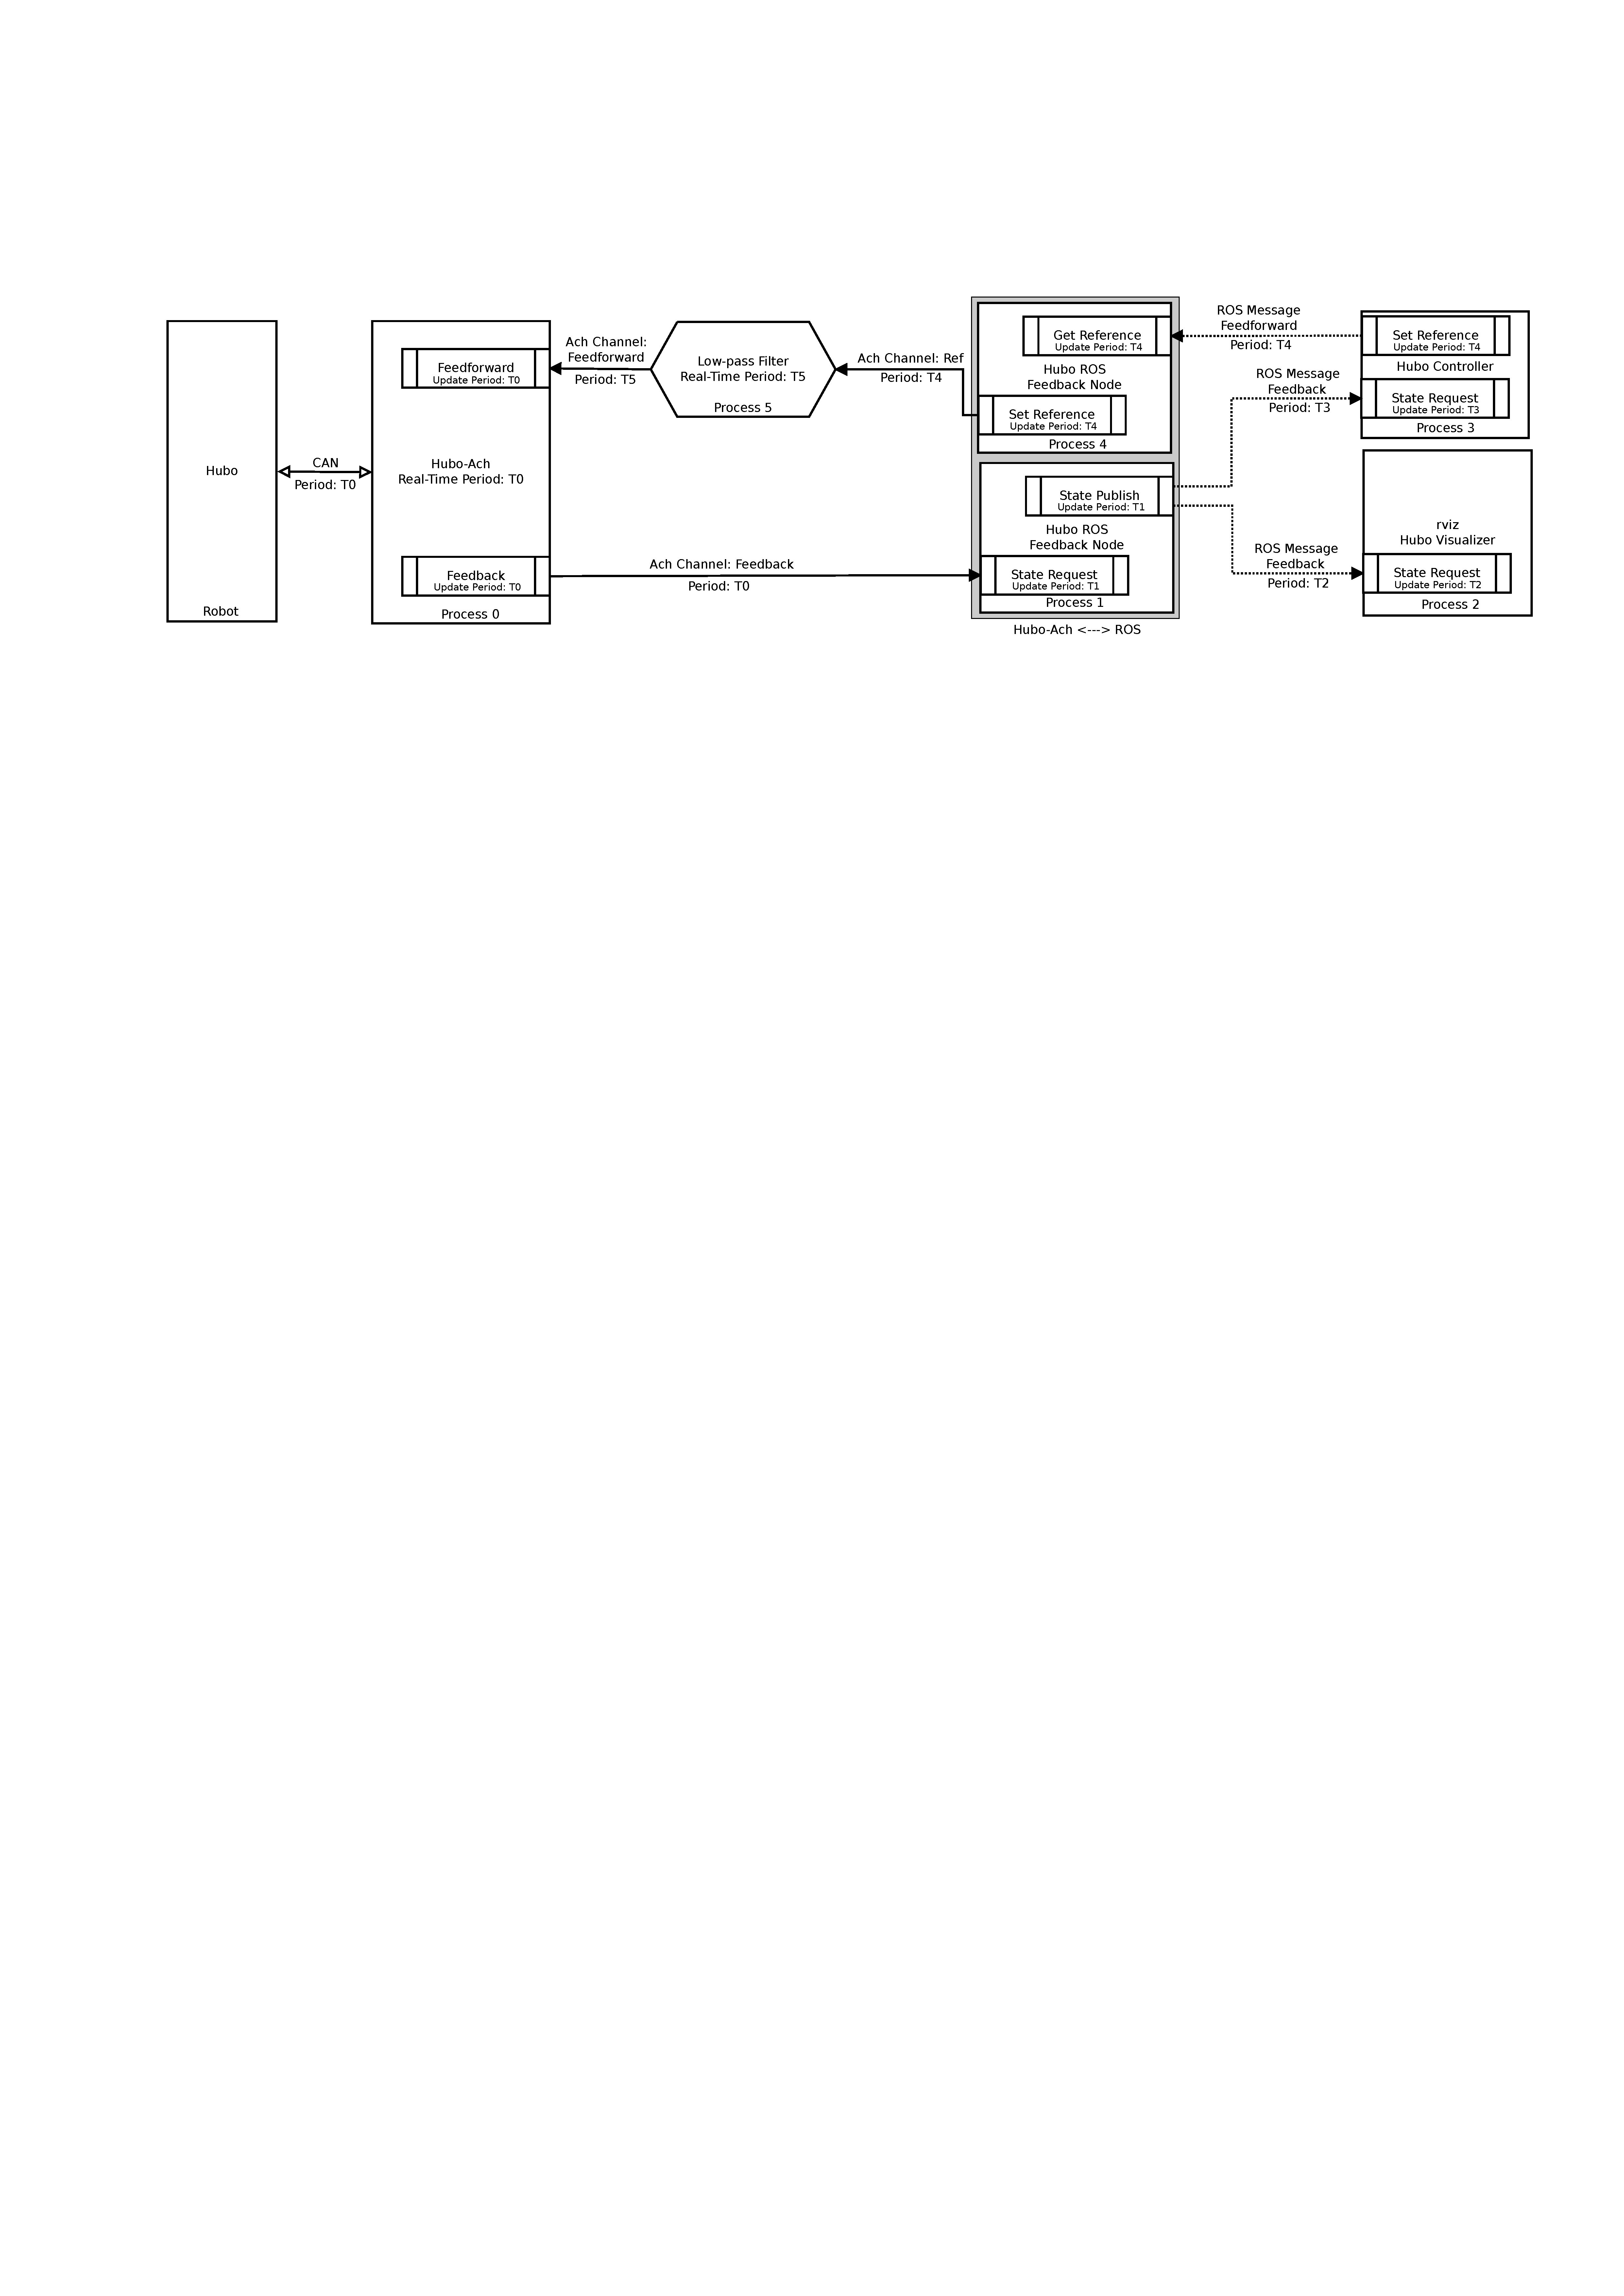
\includegraphics[width=2.0\columnwidth]{./pix/hubo-ach-diagram-ros.pdf}
%   \caption{Hubo-Ach.}
%   \label{fig:graph}
% \end{figure*}
%\definecolor{nodecolor}{RGB}{238,232,170} % light goldenrod
\begin{figure*}
  \centering
  \begin{tikzpicture}
    \node[fill=bgcolor,rounded corners=1em,draw=black,minimum
    width=\textwidth] {
  \begin{tikzpicture}[fill=white, rounded
    corners=0em,draw=black,minimum width=1em]
    \tikzstyle{proc} = [rectangle,minimum height=2.0em,minimum
    width=2.00em, font=\small,draw=black, node distance=72pt,fill=nodecolor]
    \tikzstyle{ros} = [rectangle,minimum height=2.0em,minimum
    width=2.00em, font=\small,draw=black,fill=nodecolor]
    \tikzstyle{ach} =[->, >=stealth,thick,color=black]
    \tikzstyle{ros} =[->, >=stealth,thick,dotted,color=black]
    \tikzstyle{can} =[<->, >=stealth,thick,color=green]
    \tikzstyle{lbl} =[font=\footnotesize,color=black];
    \tikzstyle{keylabel} = [node distance=1.5em]

    \node[proc,,name=achros,xshift=0]{{\tt hubo-ach-ros}};


    \node[proc,right of=achros,name=filter,xshift=0pt]{{\tt filter}};
    \node[proc,right of=filter,name=hubod,xshift=0pt]{{\tt
        hubo-daemon}}; \node[name=hardware,draw=black,right
    of=hubod,xshift=72pt,yshift=-18pt,fill=white]{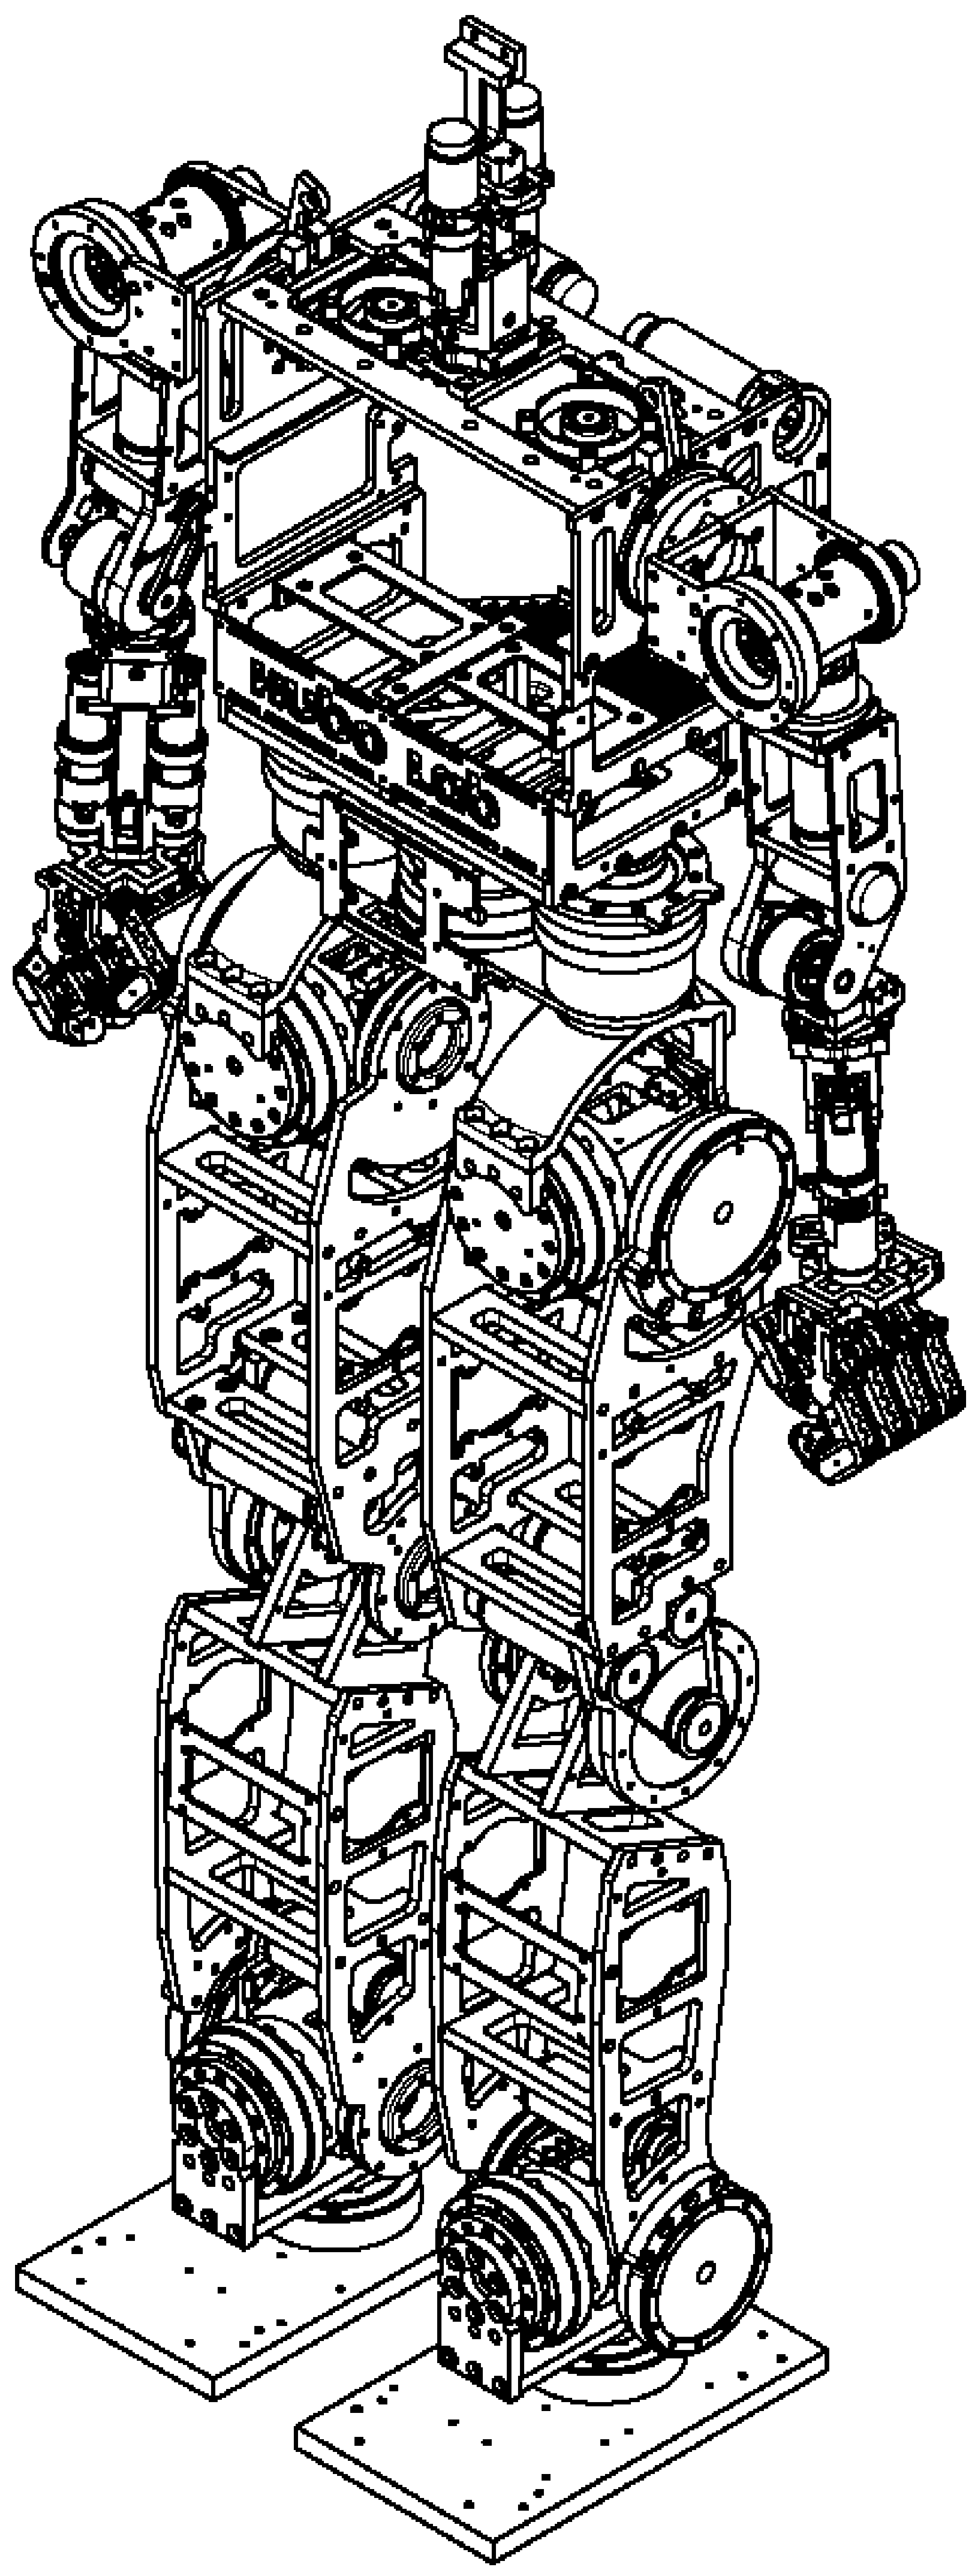
\includegraphics[height=72pt]{pix/hubo-iso}};

    \path(hubod) edge[can] node[above,lbl]{CAN}
    ($(hardware.west)+(0,18pt)$);
    \path (filter) edge[ach] node[above,lbl,yshift=10pt]{\tt feedforward} (hubod);
    \path (achros) edge[ach] node[above,lbl,yshift=10pt]{\tt ref} (filter);

    \draw[thick,->] (hubod) -- ++(0,-36pt) -- node[lbl][above]{\tt
      feedback} ++(-134pt,0)  -- ($(achros.south) + (10pt,0)$) ;

    \node[proc,name=planner,left of=achros,xshift=-36pt] {\tt planner};
    \node[proc,name=rviz,below of=planner,yshift=36pt] {\tt rviz};

    %\draw[ros] ($(achros.south west)$)  -- ($(controller.south east)$);

    \draw[ros] ($(achros.south)+(-10pt,0)$)  --
    ($(rviz)+(72pt,0)+(26pt,0)$) -- node[lbl,above]{\tt rFeedback} (rviz);
    \draw[ros] ($(rviz)+(20.0pt,-.25pt)$) -- ++(0,26pt);

    \path (planner) edge[ros] node[above,lbl,yshift=10pt] {\tt rFeedforward} (achros);


    \node[right of=hardware,name=key,xshift=3em,yshift=36pt] {Key};
    \node[keylabel,below of=key,name=can,xshift=1em] {CAN};
    \node[keylabel,below of=can,name=ach] {Ach};
    \node[keylabel,below of=ach,name=ros] {ROS};

    \path ($(key)+(-24pt,-1.5em)$) edge[can] (can);
    \path ($(key)+(-24pt,-3em)$) edge[ach] (ach);
    \path ($(key)+(-24pt,-4.5em)$) edge[ros] (ros);
  \end{tikzpicture}
  };
  \end{tikzpicture}
  \caption{Feedback loop integrating Hubo-Ach with ROS}
  \label{fig:huboachros}
\end{figure*}


%   It was
% designed by Daniel M. Lofaro\footnote{Daniel M. Lofaro:
%   http://danlofaro.com/} and Neil Dantam in collaboration with the
% \textit{Drexel Autonomous Systems Lab} at Drexel University and
% \textit{Golems - The Humanoid Robotics Laboratory}\footnote{Golems -
%   The Humanoid Robotics Laboratory: www.golems.org/} at the Georgia
% Institute of Technology.

Hubo-Ach \footnote{Available under permissive license,
  \url{http://github.com/hubo/hubo-ach}} is an Ach-based interface to Hubo's
sensors and motor controllers.  This provides a conventional GNU/Linux
programming environment, with the variety of tools available therein,
for developing applications on the Hubo.  It also efficiently links
the embedded electronics and real-time control to popular frameworks
for robotics software: ROS \cite{Quigley09},
OpenRAVE,\footnote{OpenRAVE: http://openrave.org/} and
MATLAB\footnote{MATLAB: http://www.mathworks.com/}.

%  The overarching
% goal of the Hubo-Ach system is to create an easy to use interface
% between the Hubo's electro-mechanical hardware and its programming
% environment.  System design decisions were made with the programmers
% and developers of the Hubo in mind.  This design philosophy
% streamlines closed-loop controller implementation, human robot
% interaction development and the utilization of popular robot related
% systems such as ROS\footnote{ROS: http://www.ros.org/} (Robot
% Operating System), OpenRAVE\footnote{OpenRAVE: http://openrave.org/}
% and MATLAB\footnote{MATLAB: http://www.mathworks.com/} on the Hubo
% platform.

Reliability is a critical issue for software on the Hubo.  As a
bipedal robot, Hubo must constantly maintain dynamic balance; if the
software fails, it will fall and break.  A multi-process software
design improves Hubo's reliability by isolating the critical balance
code from other non-critical functions, such as control of the neck or
arms.  For the high-speed, low-latency communications and priority
access to latest sensor feedback, Ach provides the underlying IPC.

% The inherent complex nature
% and instability of humanoids means the controller is required to be
% active at all times.  Thus the Hubo-Ach system must be immune to
% crashes due to unstable software interfacing with the system.  Our
% solution is to separate Hubo-Ach and the controllers into stand-alone
% processes with the ability to \textit{``talk to each other''} through
% inter process communications also known as IPC.  This allows for one
% or more controllers to crash and not cause Hubo-Ach or other the
% controller processes to fail as well.  Closed-loop control of the Hubo
% requires high-speed, low-latency communications.  Priority access to
% the most recent state data (i.e. sensor feedback) is needed.  The IPC
% called Ach \cite{ach} fit all of the above criteria and thus was used
% for the inter process communications for the Hubo-Ach system.

Hubo-Ach handles CAN bus communication between the PC and embedded
electronics.  Because the motor controllers synchronize to the control
period in a \emph{phase lock loop} (PLL), the single {\tt hubo-daemon}
process runs at a fixed control rate and communicates on the bus.  The
embedded controllers lock to this rate and linearly interpolate
between the commanded positions, providing smoother trajectories in
the face of limited communication bandwidth.  This communication
process also avoids bus saturation; with CAN bandwidth of 1 Mbps and
200Hz control rate, {\tt hubo-daemon} currently utilizes 78\% of the
bus.  {\tt Hubo-daemon} receives position targets from a
{\tt feedforward} channel and publishes sensor data to the
{\tt feedback} channel, providing the direct software interface to
the embedded electronics.

% Hubo-Ach runs as a daemon performing a real-time (RT) loop in the
% background of a Linux based system.  Via the CAN bus the Hubo-Ach
% daemon sets all references to the motor controllers at the rising edge
% of the RT loop then requests the state data from the sensors.  The
% references are taken from the most recently published
% \textbf{Feedforward} Ach channel.  The state data is published to the
% \textbf{Feedback} Ach channel.  All of the data in the
% \textbf{Feedforward} and \textbf{Feedback} Ach channels are in
% \textit{SI} units.  The RT loop runs with a period of $T_0$ which is
% currently set to 5.0 $ms$.  The RT loop in Hubo-Ach is needed to
% ensure the internal phase-locked loop (PLL) of the motor controllers
% lock onto the reference update rate and timing.  Within the motor
% controllers the PLL is used to perform linear interpolation between
% reference commands.  This helps reduce the \textit{jerk} on each of
% the high-gain PID controlled joints.  In addition the RT loop is used
% to ensure the CAN bus's bandwidth is not saturated.  The CAN bus
% bandwidth is 1.0 $Mbps$ and Hubo-Ach currently utilizes is 78\% of it.


Each Hubo-Ach controller is an independent processes.  The controllers
handle tasks such as balance, manipulation, and human-robot
interaction.  Each controller asynchronously reads state from the {\tt
  feedback} Ach channel and sets reference positions in the {\tt
  feedforward} channel.  {\tt Huobo-daemon} reads the most recent
reference position from the {\tt feedforward} channel on the the
rising edge of its control cycle.  This allows the controller
processes to run at arbitrary rates without effecting the PLL of the
embedded motor controllers or the CAN bus bandwidth utilization.




\autoref{fig:huboachros} shows an example control loop integrating
Hubo-Ach and ROS.  The {\tt hubo-daemon} communicates with the
embedded controllers at $200 \hertz$, publishing to the {\tt feedback}
channel.  The {\tt hubo-ach-ros} process bridges ROS topics and Ach
channels.  It translates messages on the {\tt feedback} Ach channel to
the {\tt rFeedback} ROS topic and translates the {\tt rFeedforward}
ROS topic to the {\tt ref} Ach channel.  The {\tt planner} process
computes desired trajectories, which are relayed via {\tt
  hubo-ach-ros} to {\tt filter} for preprocessing to smooth the motion
and reduce \emph{jerk} before {\tt hubo-daemon} communicates
references to the embedded controllers.  During operation, {\tt rviz}
displays a 3D model of the Hubo's current state.  Each of these
process runs asynchronously, communicating at different rates;
however, {\tt hubo-ach-daemon} maintains its $200 \hertz$ cycle,
ensuring phase lock with the embedded controllers.  This control loop
effectively integrates real-time IPC and control under Hubo-Ach with
the non-real-time ROS environment.

% \textit{Process 2} is the feedforward portion of the
% Hubo-Ach to ROS and ROS to Hubo-Ach bridge.  It reads the
% \textit{aFeedback} channel at given rate and publishes the data to the
% ROS topic \textit{\textbf{Feedback}}.  The data published is the state
% data found in \textbf{aFeedback} at the time it was read.  The rate it
% is read at can be the same or different from that of \textit{Process
%   1} and does not have to be regular.  \textit{Process 2} is a Hubo
% visualizer that reads the state data off of the ROS topic
% \textbf{rFeedback} and applies it to the OpenHUBO model in rviz.
% \textit{Process 3} is the closed loop controller.  It takes in the
% state data from the \textbf{rFeedback} ROS topic, performs a control
% such as visual servoing, impedance control, path-planning etc.  The
% resulting joint space references are published to the
% \textbf{rFeedforward} ROS topic.  \textit{Process 4} is event based
% where when a new message is posted on \textbf{rFeedforward} the second
% part of the Hubo-Ach to ROS and ROS to Hubo-Ach bridge it posts the
% references in the ROS message to the \textbf{aRef} Ach Channel.  To
% allow step inputs to be commanded to the robot without damaging the
% joints a low-pass filter is added between ROS and the Hubo-Ach daemon
% \textit{Process 5}.  This filter reduces the \textit{jerk} on each
% joint.  The resulting filtered reference is posted to the
% \textbf{aFeedforward} Ach channel where the Hubo-Ach daemon can read
% it and command the Hubo.

Hubo-Ach is in use for numerous projects at several research labs.
Users include include groups at MIT, WPI, Ohio State, Purdue,
Swarthmore College, Georgia Tech, and Drexel University.  These
projects primarily revolve around the DARPA Robot Challenge
(DRC)\footnote{DARPA Robot Challenge:
  http://www.theroboticschallenge.org/} team
DRC-Hubo\footnote{DRC-Hubo Homepage: http://drc-hubo.com/}.  The DRC
includes rough terrain walking, ladder climbing, valve turning,
vehicle ingress/egress and more.  \autoref{fig:valve} shows the Hubo
using the Hubo-Ach system to turn a valve.

%   The video of the valve
% turning example can be found at http://drc-hubo/video/valve-example/.

Hubo-Ach provides an effective base for developing real-time
applications on the Hubo.  Separating software modules into different
processes increases system reliability.  A failed process can be
independently restarted, minimizing chance of damage to the robot.  In
addition, the controllers can run at fast rates because Ach provides
high-speed low-latency communication with {\tt hubo-daemon}.  Hubo-Ach
provides a C API that is easily called from high-level programming
languages and integrates with popular platforms for robot software
such as ROS and MATLAB, providing additional development flexibility.
Hubo-Ach is a validated and easy to use interface between the
mechatronics and the software control algorithms of the Hubo full-size
humanoid robot.

% The key point is that Hubo-Ach updates the state data in the
% \textbf{aFeedback} channel and commands the motors with the references
% set in the \textbf{aFeedforward} channel in real-time.

%%% Local Variables:
%%% mode: latex
%%% TeX-master: "ach"
%%% End:

\section{Inter Process Comunication Comparision}\label{sec:ipc}
	POSIX provides three main types of IPC: streams, datagrams and shared memory.  
A review of each is made before making a choice for desired message passing skeam.

\noindent \textbf{Streams:}\\
The IPC type \textit{stream} includes pipes, FIFOs, stream sockets, and TCP sockets.
All stream basted methods suffer from head of line (HOL) blocking which means older data \textbf{must} be read before newer data.
%In addition all streaming methods are exposed to file abstraction (read/write byte sequence).
For robotic applications we must be able to access the newest data imediately and read older data if needed.
This is a different paradime then typical streaming application because robots are real-time sensitive meaning the newest information holds more value to the overall system than the older data.

\noindent \textbf{Datagrams:}\\
POSIX \textit{datagrams} come in two major flavors, \textit{datagram sockets} and \textit{POSIX message queues}.
Datagram sockets are less likely to block the sender then streams.
The most important reason why datagrams are \textbf{not} a good solution for my application is that newer messages are lost if the buffer is filled.
Newer data is more important than older data in my control system thus this is not a viable option.

POSIX message queues are simular to datagrams sockets with the addition of message priorities.
Unlike datagram sockets if the buffer fills the POSIX message queues will block.
This will cause the application to stop processing until it is able to read/flush the old messages.
Thus simular to other methods mentioned this also suffers from HOL.

\noindent \textbf{Shared Memory:}\\
POSIX shared memory is very fast and allows access to the latest data by simply writing over a variable.
Though I have been advicating that the newest information is the most important, old information can not be discarded.
If using POSIX shared memory there is no way of recovering older data that might have been missed by a controller.

What is needed is a method of sharing data that is \textit{non-blocking} and as \textit{low-latancy} like shared memory, but still holds older data and uses an asyncronous IO scheme.
The asyncronous IO scheme is required so the controller is not locked to a set rate by the data transactionn method.
N. Dantam et. al.\cite{ach} shows that Asynchronous IO (AIO) might be approperiate for this application however the implimentaiton under Linux is not as mature as I require.
In addition N. Dantam shows that other IPC mechanism using select/poll/epoll/kqueue are widely used network server and help midigate but not totally removed the issue of HOL.
The primary problem being that that thought the sender will not block the reader must stil read the oldest data first.
The question now is what IPC mechanism will be suitable for my control system.

Upon investigation three major mechanisms are avaliable; Robot Operating System (ROS)\cite{ros}, Message Passing Interface (MPI)\cite{Gropp:1999:UMP:330577} and Ach\cite{ach}.
Though ROS 

\section{Timing}\label{sec:timing}
	\begin{figure}
\centering

\begin{tikzpicture}[->,>=stealth',shorten >=1pt,auto,node distance=5cm,
  thick,main node/.style={fill=white!20,draw,font=\sffamily\footnotesize\bfseries}]

  
  \node[main node] (latesRef) [ text width=2.0cm, minimum height=1.5cm, align=center]   {Reference\\(Latest)};
  \node[main node] (ctrl)     [left=0.8cm of latesRef,minimum height=2.5cm, align=center]                           {Controller};
  \node[main node] (getRef)   [right=1.5cm of latesRef, text width=3.0cm, minimum height=1.1cm, align=center]      {Get Reference};
 

 % \node[main node] (fromsim)     [above=1.0cm of getRef, text width=3.0cm, minimum height=1.1cm, align=center]    {From Simulator\\ Hold (sim mode)};
 % \node[main node] (sim)         [above=1.0cm of fromsim, text width=3.0cm, minimum height=1.1cm, align=center]    {Simulator \\Trigger\\ (sim mode)};

 \node[main node, draw=white] (haname2)   [above=0.2cm of getRef, align=center]   {};

  \node[main node] (dodebug)     [below=1.0cm of getRef, text width=3.0cm, minimum height=1.1cm, align=center]    {User Commands\\ (debug)};
  \node[main node] (tosim)       [below=1.0cm of dodebug, text width=3.0cm, minimum height=1.1cm, align=center]    {To Simulator\\ Trigger};
  \node[main node] (filter)      [below=1.0cm of tosim, text width=3.0cm, minimum height=1.1cm, align=center]     {Filter};
  \node[main node] (setRef)      [below=1.0cm of filter, text width=3.0cm, minimum height=1.1cm, align=center]    {Set Reference};
  \node[main node] (reqSens)     [below=1.0cm of setRef, text width=3.0cm, minimum height=1.1cm, align=center]    {Request Sensors};
  \node[main node] (getSens)     [below=1.0cm of reqSens, text width=3.0cm, minimum height=1.1cm, align=center]   {Get Sensors};
  \node[main node] (canWait)     [below=1.0cm of getSens, text width=3.0cm, minimum height=1.1cm, align=center]   {Wait on CAN};
  \node[main node] (putState)    [below=1.0cm of canWait, text width=3.0cm, minimum height=1.1cm, align=center]   {Put State};
  \node[main node] (rthold)      [left=0.5cm of getSens, minimum height=1.1cm, align=center]   {Real-Time\\Hold};



  \node[main node] (latestState) [left=1.5cm of putState, text width=2.0cm, minimum height=1.1cm, align=center, yshift=-1.0cm]   {State\\(Latest)};
  \node[main node, draw=white] (haname)   [right=3.0cm of putState, align=center]   {};

  \node[main node] (robot)    [right=4.8cm of getSens, minimum height=5.5cm, align=center]    {Robot};
  

%H_ref.ref[jnt] = deg;
%H_ref.mode[jnt] = HUBO_REF_MODE_ENC_FILTER;

  \path[->, dashed,every node/.style={font=\sffamily\small}]
    (ctrl) edge node [above] {} (latesRef);

%  \path[->, every node/.style={font=\sffamily\small}]
%    (fromsim) edge node [right] {$t_0=0.011~ms$} (getRef);
%\draw[->] ([xshift=-1.2 cm]fromsim.south)  to [out=-90,in=90] node [right] {$t_0=0.011~ms$} ([xshift=-1.2 cm]getRef.north)  ;
%\draw[->] ([xshift=-1.2 cm]getRef.south)   to [out=-90,in=90] node [right] {$t_1=0.011~ms$} ([xshift=-1.2 cm]tosim.north)  ;
%\draw[->] ([xshift=-1.2 cm]tosim.south)   to [out=-90,in=90] node [right] {$t_2=0.011~ms$} ([xshift=-1.2 cm]filter.north)  ;
%\draw[->] ([xshift=-1.2 cm]filter.south)   to [out=-90,in=90] node [right] {$t_3=???~ms$} ([xshift=-1.2 cm]setRef.north)  ;
%\draw[->] ([xshift=-1.2 cm]setRef.south)   to [out=-90,in=90] node [right] {$t_4=???~ms$} ([xshift=-1.2 cm]reqSens.north)  ;
%\draw[->] ([xshift=-1.2 cm]reqSens.south)   to [out=-90,in=90] node [right] {$t_5=???~ms$} ([xshift=-1.2 cm]getSens.north)  ;
%\draw[->] ([xshift=-1.2 cm]getSens.south)   to [out=-90,in=90] node [right] {$t_6=0.011~ms$} ([xshift=-1.2 cm]putState.north)  ;
%\draw[->] ([xshift=0.0 cm]putState.west)   to [out=180,in=-90] node [below, yshift=-0.5cm, xshift=-0.2cm] {$t_7=0.011~ms$} ([xshift=0.0 cm]rthold.south)  ;


\draw[->] ([xshift=0.0cm]latesRef.east)  to [out=0,in=-180]  node [right]  {} ([xshift=0.0cm]getRef.west)  ;
%\draw[->] ([xshift=0.0cm]fromsim.south)  to [out=-90,in=90]  node [right]  {} ([xshift=0.0cm]getRef.north)  ;
\draw[->] ([xshift=0.0cm]getRef.south)   to [out=-90,in=90]  node [right]  {} ([xshift=0.0cm]dodebug.north)  ;
\draw[->] ([xshift=0.0cm]dodebug.south)  to [out=-90,in=90]  node [right]  {} ([xshift=0.0cm]tosim.north)  ;
\draw[->] ([xshift=0.0cm]tosim.south)    to [out=-90,in=90]  node [right]  {} ([xshift=0.0cm]filter.north)  ;
\draw[->] ([xshift=0.0cm]filter.south)   to [out=-90,in=90]  node [right]  {} ([xshift=0.0cm]setRef.north)  ;
\draw[->] ([xshift=0.0cm]setRef.south)   to [out=-90,in=90]  node [right]  {} ([xshift=0.0cm]reqSens.north)  ;
\draw[->] ([xshift=0.0cm]reqSens.south)  to [out=-90,in=90]  node [right]  {} ([xshift=0.0cm]getSens.north)  ;
\draw[->] ([xshift=0.0cm]getSens.south)  to [out=-90,in=90]  node [right]  {} ([xshift=0.0cm]canWait.north)  ;
\draw[->] ([xshift=0.0cm]canWait.south)  to [out=-90,in=90]  node [right]  {} ([xshift=0.0cm]putState.north)  ;
\draw[->] ([xshift=0.0 cm]putState.west) to [out=180,in=-90] node [below, yshift=-0.5cm, xshift=-0.2cm] {} ([xshift=0.0 cm]rthold.south)  ;
\draw[->] ([xshift=0.0 cm]rthold.north)  to [out=90,in=-120] node [left, yshift=-1.0cm, xshift=-0.8cm, rotate=90] {} ([xshift=0.0 cm]getRef.west)  ;
\draw[->] ([xshift=0.0cm]putState.south) to [out=-90,in=0]   node [right]  {} ([xshift=0.0cm]latestState.east)  ;




%\draw[->] ([yshift=0.75cm]fromsim.east)  to [out=-30,in=30] node [right] {$t_0=0.014~ms$} ([yshift=-0.75cm]fromsim.east)  ;
\draw[->] ([yshift=0.75cm]getRef.east)  to [out=-30,in=30] node [right] {$t_0=0.010~ms$} ([yshift=-0.75cm]getRef.east)  ;
\draw[->] ([yshift=0.75cm]dodebug.east)  to [out=-30,in=30] node [right] {$t_1=0.011~ms$} ([yshift=-0.75cm]dodebug.east)  ;
\draw[->] ([yshift=0.75cm]tosim.east)  to [out=-30,in=30] node [right] {$t_2=0.014~ms$} ([yshift=-0.75cm]tosim.east)  ;
\draw[->] ([yshift=0.75cm]filter.east)  to [out=-30,in=30] node [right] {$t_3=0.008~ms$} ([yshift=-0.75cm]filter.east)  ;
\draw[->] ([yshift=0.75cm]setRef.east)  to [out=-30,in=30] node [right] {$t_4=0.152~ms$} ([yshift=-0.75cm]setRef.east)  ;
\draw[->] ([yshift=0.75cm]reqSens.east)  to [out=-47,in=47] node [right] {$t_5=1.365~ms$} ([yshift=-0.75cm]getSens.east)  ;
\draw[->] ([yshift=0.75cm]canWait.east)  to [out=-30,in=30] node [right,align=center] {$t_6=3.000~ms$\\(hard timeout)} ([yshift=-0.75cm]canWait.east)  ;
%\draw[->] ([yshift=0.75cm]reqSens.east)  to [out=-30,in=30] node [right] {$t_5=???~ms$} ([yshift=-0.75cm]reqSens.east)  ;
%\draw[->] ([yshift=0.75cm]getSens.east)  to [out=-30,in=30] node [right] {$t_6=???~ms$} ([yshift=-0.75cm]getSens.east)  ;
\draw[->] ([yshift=0.75cm]putState.east)  to [out=-30,in=30] node [right] {$t_7=0.092~ms$} ([yshift=-0.75cm]putState.east)  ;
\draw[->] ([yshift=-0.75cm]rthold.west)  to [out=120,in=-120] node [above, yshift=1.5cm, xshift=0.3cm, rotate=90] {$\displaystyle t_{hold}=T-\sum_{i=0}^{8} t_i=0.348~ms$} ([yshift=0.75cm]rthold.west)  ;

\draw[->, dashed] ([xshift=0.0cm]latestState.west)   to [out=120,in=-90] node [right] {} ([xshift=0.0cm]ctrl.south)  ;
%\draw[->, dashed] ([xshift=0.0cm]sim.south)   to [out=-90,in=90] node [right] {} ([xshift=0.0cm]fromsim.north)  ;

\node[fit=(getRef)(putState)(rthold)(haname)(latestState)(haname2), draw,label={south:Hubo-Ach}] (hubo-ach) [minimum width=4.5cm] {};



\draw[->,loosely dotted] ([xshift=0.75cm]setRef.south)  to [out=-30,in=-180] node [above] {} ([yshift=1.50cm]robot.west)  ;
\draw[->,loosely dotted] ([xshift=0.75cm]reqSens.south)  to [out=-30,in=-180] node [above] {} ([yshift=0.75cm]robot.west)  ;
\draw[<-,loosely dotted] ([xshift=0.0cm]getSens.east)  to [out=0,in=-180] node [above, xshift=1.7cm] {CAN} ([yshift=0.0cm]robot.west)  ;
\draw[<-,loosely dotted] ([xshift=0.75cm]canWait.north)  to [out=30,in=-180] node [above] {} ([yshift=-0.75cm]robot.west)  ;




%  \path[->,every node/.style={font=\sffamily\small}]
%    (ik) edge node [above] {$\overline{\theta_d}$} (filter);

% \draw[->] ([xshift=-0.5 cm]filter.south)  -- node [left] {$\overline{\theta_r}$} ([xshift=-0.5 cm]hubo-ach.north)  ;
% \draw[->] ([xshift=0.5 cm]hubo-ach.north) -- node [left] {$\overline{\theta_a}$} ([xshift=0.5 cm]filter.south)  ;

% \path[<->,dashed, every node/.style={font=\sffamily\small}]
%    (hubo) edge node [above] {CAN} (hubo-ach);


\end{tikzpicture}
\caption{Timing diagram of Hubo-Ach.  All times $t_*$ denote measured times each block takes to complete.  Tests were done on a 1.6Ghz Atom D525 Dual Core with 1GB DDR3 800Mhz memory running Ubuntu 12.04 LTS linux kernel 3.2.0-29 on a Hubo2+ utilizing a CAN bus running at 1Mbps baud.  Average CPU usage is 7.6\% using a total of 4Mb or memory.}
\label{fig:hubo-ach-timing}
\end{figure}


To ensure that the Hubo-Ach controller is able to run at the desired control rates, timing experiments of each part of the controller was taken.
All tests were done with a sample step size of $0.005~sec$.
Each of the following figures have the same X and Y scale.
This is to give a visual representation of how much each portion of the cycle each part of Hubo-Ach takes up.




Fig.~\ref{fig:timing-getRef} shows the amount of time it takes to request and get the reference for the actuators.
This reads the most recent reference off of the feedforward channel and uses that as the reference used in this cycle of Hubo-Ach.
This time is measured to be $0.0010~ms$ with micro-second accuracy.
The standard deviation is $0.0028$.



Fig.~\ref{fig:timing-doCmd} shows the amount of time it takes to complete all unread commands given by the user via the console.
User commands are manual actions such as homing individual or all joints, resetting actuator errors, and reading error states.
This time is measured to be $0.011~ms$ with micro-second accuracy.
The standard deviation is $0.0.0033$.


Fig.~\ref{fig:timing-getTrigger} shows the amount of time it takes to send the external trigger.  
This external trigger tells a controller or simulator when the new reference's and commands have been read.
In real-time mode the measured time delay is $0.0014~ms$ with micro-second accuracy and a standard deviation of $0.0035$.


Fig.~\ref{fig:timing-filter} shows the amount of time it takes to process the built in filter.
This filter has multiple options:
\begin{itemize}
\item Direct reference mode where the filter acts as a reference pass through (Section~\ref{sec:singlejointStep}).
\item Low pass filter based on previous reference commands (Section~\ref{sec:singlejointFilter}).
\item Low pass filter using feedback from the actual position of the joint (Section~\ref{sec:singlejointEnc}).
\item Compliance amplification mode which artificially increases the compliance of the joint (Section~\ref{sec:singlejointRefComplience})
The measured time delay is $0.0080~ms$ with micro-second accuracy.
The standard deviation is $0.0030~ms$.
\end{itemize}
This gives the system the option of reducing the jerk on the high-gain position controlled actuators allowing for slower update rates on the reference channel.
The \textit{direct reference} mode allows a controller to have direct access to the commanded reference with no additional filtering.





Fig.~\ref{fig:timing-setRef} shows amount of time it takes to set the reference on the actuators via setting the data in the CAN bus buffer.
The amount of time it takes for the for the references to be set to the actuators via the CAN is dependent on the baud rate of the CAN bus.
Currently the baud rate is set to 1Mbps.
CAN is the limiting factor in the loop rate.
The table of the required bits to be sent via can is available in Table~\ref{table:huboCAN}.



\begin{sidewaystable}
\scriptsize
\caption{Hubo CAN packet data length and explanation}
\begin{tabular}{p{2cm} || p{1cm} | p{3cm} | p{1cm} | p{1cm} | p{1cm} | p{1cm} | p{1cm} | p{1cm}| p{1cm} | p{1cm} | p{0.5cm} | p{0.5cm}}
\hline



Field name	&	Length (bits)	&	Purpose	&	Pos CMD	&	Board Status (main)	&	Board Status (Neck and finger)	&	Encoder Pos (normal)	&	Encoder Pos (Neck)	&	Encoder Pos Finger (0)	&	Encoder Pos (Finger 1)	&	Current	&	FT	&	IMU	\\ \hline 
\hline
Start-of-frame	&	1	&	Denotes the start of frame transmission	&	1	&	1	&	1	&	1	&	1	&	1	&	1	&	1	&	1	&	1	\\ \hline
Identifier	&	11	&	A (unique) identifier for the data which also represent the message priority	&	11	&	11	&	11	&	11	&	11	&	11	&	11	&	11	&	11	&	11	\\ \hline
Remote transmission request (RTR)	&	1	&	Dominant (0) (see Remote Frame below)	&	1	&	1	&	1	&	1	&	1	&	1	&	1	&	1	&	1	&	1	\\ \hline
Identifier extension bit (IDE)	&	1	&	Must be dominant (0)Optional	&	1	&	1	&	1	&	1	&	1	&	1	&	1	&	1	&	1	&	1	\\ \hline
Reserved bit (r0)	&	1	&	Reserved bit (it must be set to dominant (0), but accepted as either dominant or recessive)	&	1	&	1	&	1	&	1	&	1	&	1	&	1	&	1	&	1	&	1	\\ \hline
Data length code (DLC)*	&	4	&	Number of bytes of data (0–8 bytes)	&	4	&	4	&	4	&	4	&	4	&	4	&	4	&	4	&	4	&	4	\\ \hline
Data field	&	0–64 (0-8 bytes)	&	Data to be transmitted (length in bytes dictated by DLC field)	&	48	&	64	&	40	&	64	&	48	&	48	&	32	&	64	&	64	&	64	\\ \hline
CRC	&	15	&	Cyclic Redundancy Check	&	15	&	15	&	15	&	15	&	15	&	15	&	15	&	15	&	15	&	15	\\ \hline
CRC delimiter	&	1	&	Must be recessive (1)	&	1	&	1	&	1	&	1	&	1	&	1	&	1	&	1	&	1	&	1	\\ \hline
ACK slot	&	1	&	Transmitter sends recessive (1) and any receiver can assert a dominant (0)	&	1	&	1	&	1	&	1	&	1	&	1	&	1	&	1	&	1	&	1	\\ \hline
ACK delimiter	&	1	&	Must be recessive (1)	&	1	&	1	&	1	&	1	&	1	&	1	&	1	&	1	&	1	&	1	\\ \hline
End-of-frame (EOF)	&	7	&	Must be recessive (1)	&	7	&	7	&	7	&	7	&	7	&	7	&	7	&	7	&	7	&	7	\\ \hline
	&		&	Total	&	92	&	108	&	84	&	108	&	92	&	92	&	76	&	108	&	108	&	108	\\ \hline

\end{tabular}
\label{table:huboCAN}
\end{sidewaystable}
\normalsize



Fig.~\ref{fig:timing-getPos}, \ref{fig:timing-imu}, \ref{fig:timing-acc}, \ref{fig:timing-ft} shows the amount of time it takes to request and get the state data from the actuator from over the CAN bus.
This takes in total $1.365~ms$ plus an additional $3.0~ms$ for wait-on-CAN to ensure all queued messages in the CAN buffer are send and received. 


Fig.~\ref{fig:timing-setstate} shows the amount of time it takes to set the state to the feedback channel.
The measured delay is $0.092~ms$ with a standard deviation of $0.091$.





\begin{figure}[thpb]
  \centering
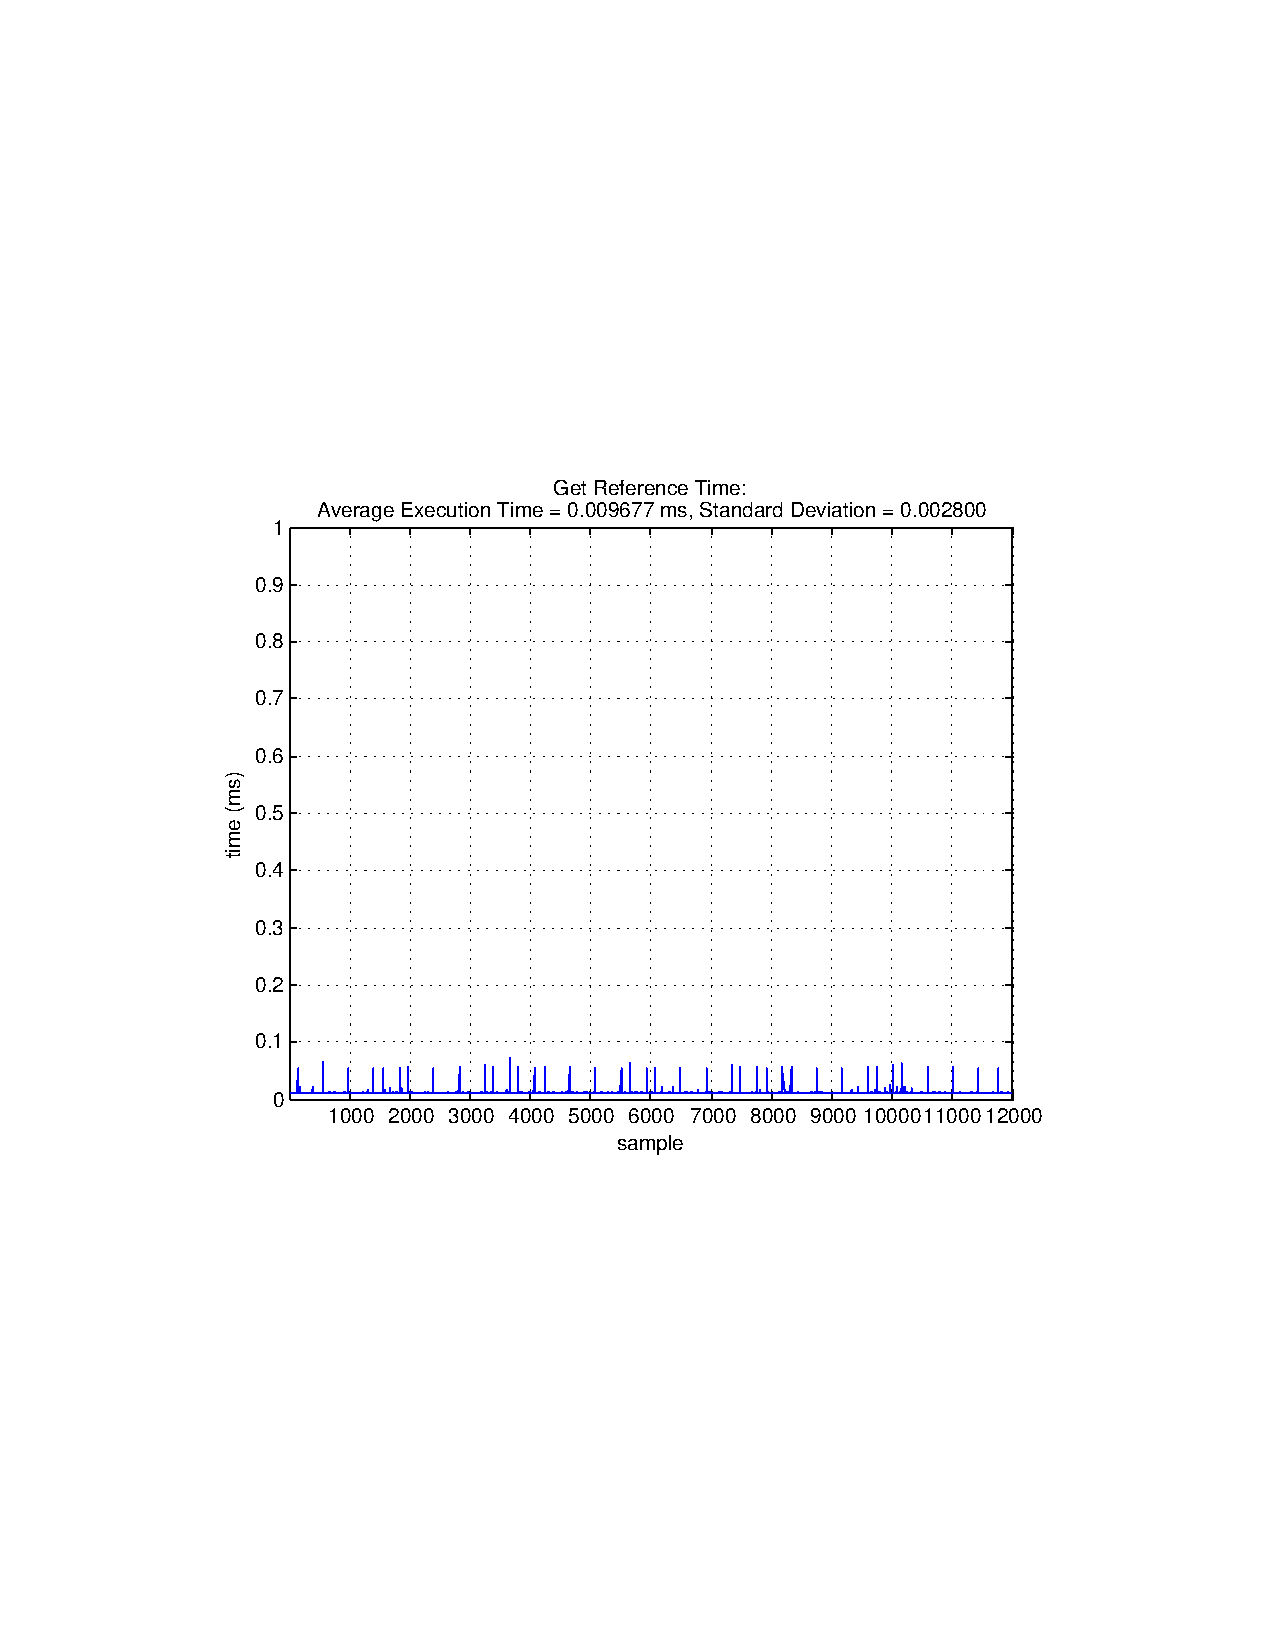
\includegraphics[width=0.6\columnwidth]{./timingData/getRef.pdf}
  \caption{The amount of time it takes to request and get the reference for the actuators.  In this case each sample has a time step of $0.005~sec$}
  \label{fig:timing-getRef}
\end{figure}


\begin{figure}[thpb]
  \centering
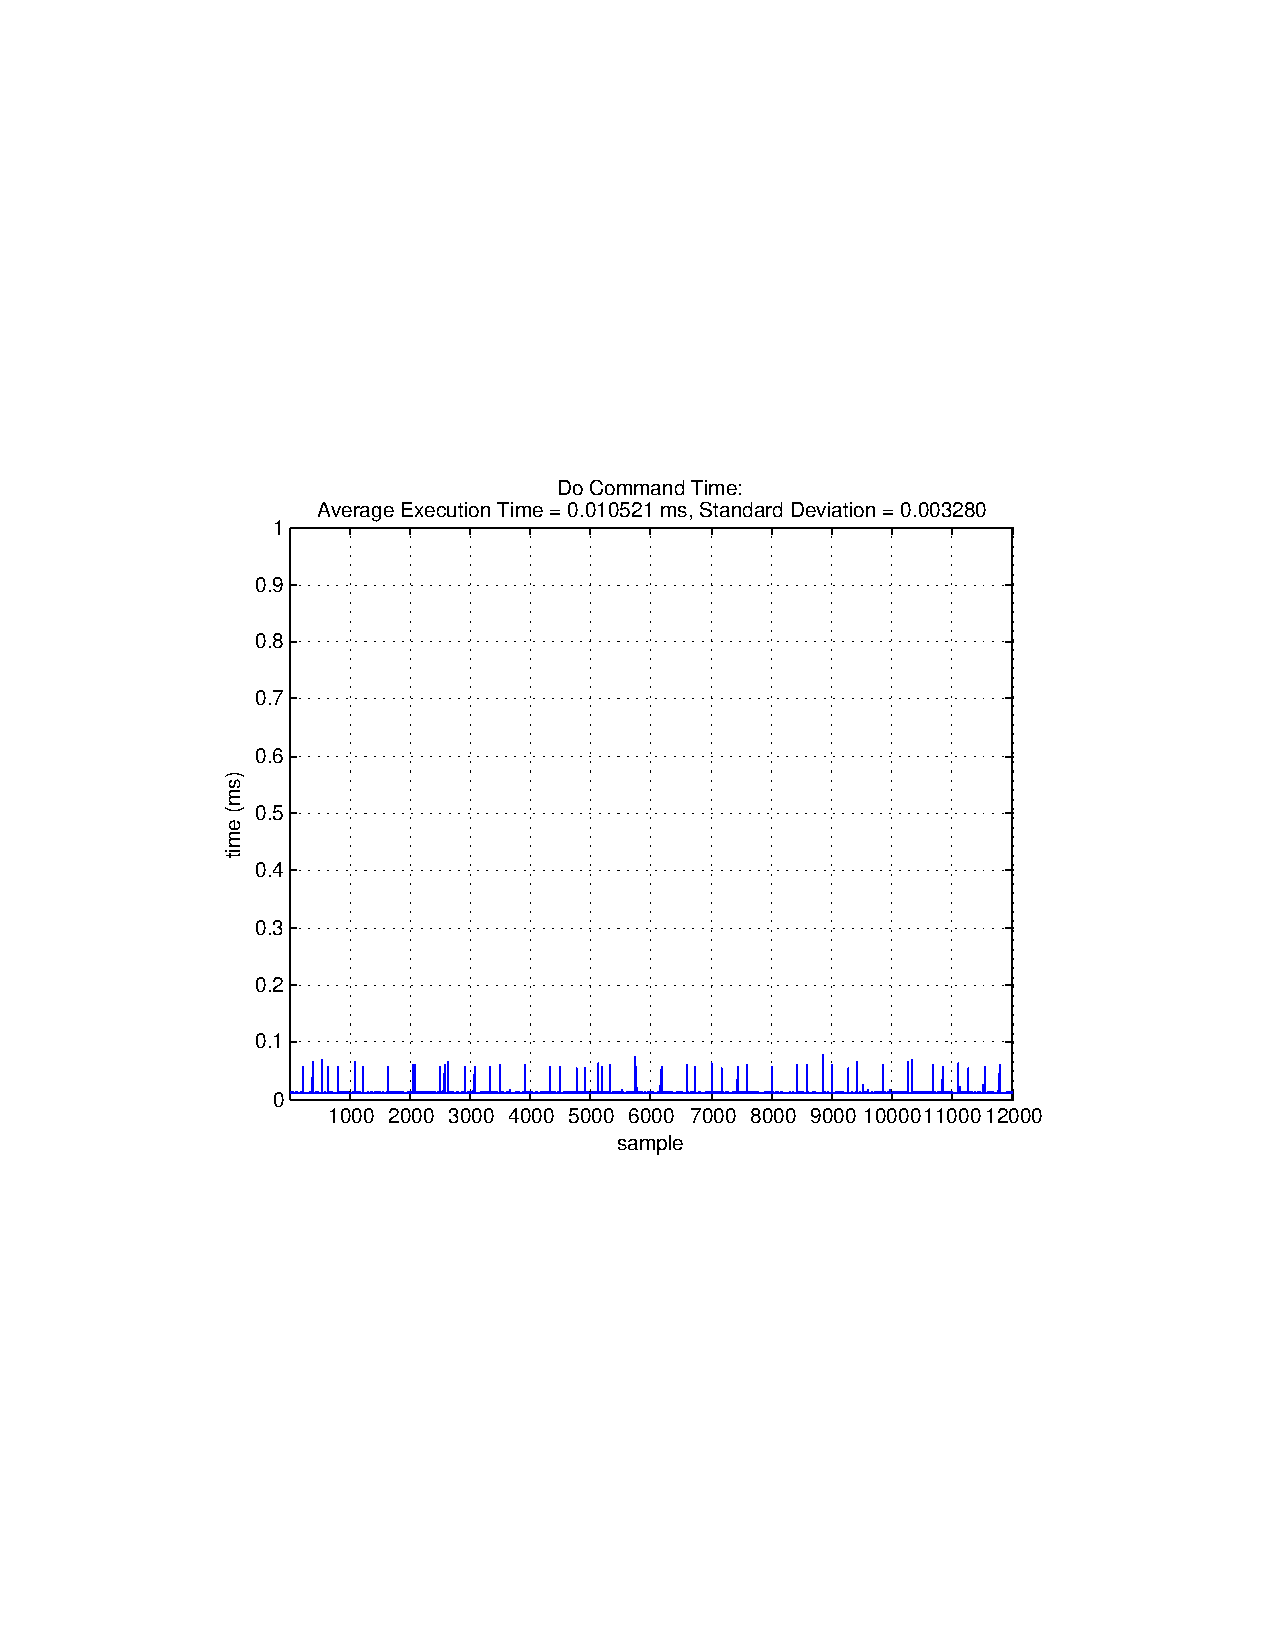
\includegraphics[width=0.6\columnwidth]{./timingData/doCmd.pdf}
  \caption{The amount of time it takes to complete all unread commands given by the user via the console.  In this case each sample has a time step of $0.005~sec$}
  \label{fig:timing-doCmd}
\end{figure}


\begin{figure}[thpb]
  \centering
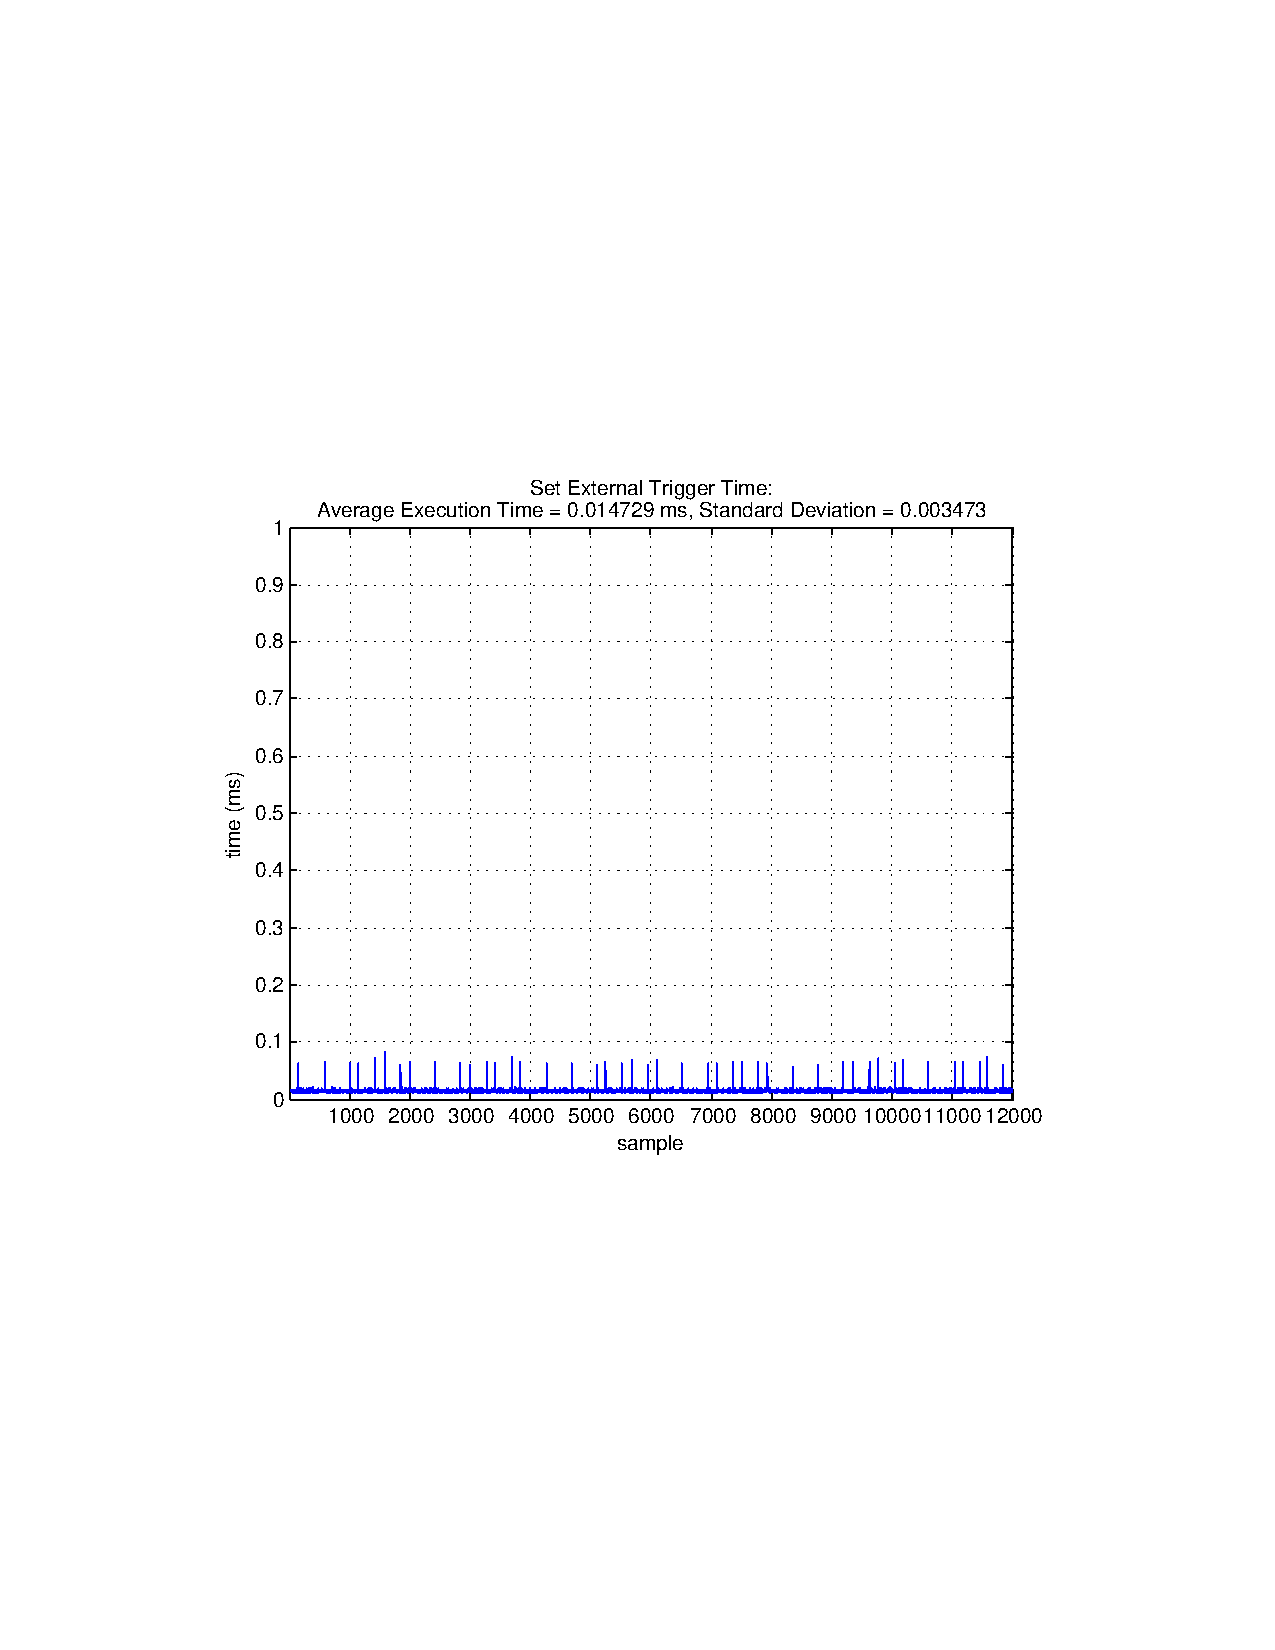
\includegraphics[width=0.6\columnwidth]{./timingData/getTrigger.pdf}
  \caption{The amount of time it takes to send the external trigger.  In this case each sample has a time step of $0.005~sec$}
  \label{fig:timing-getTrigger}
\end{figure}

\begin{figure}[thpb]
  \centering
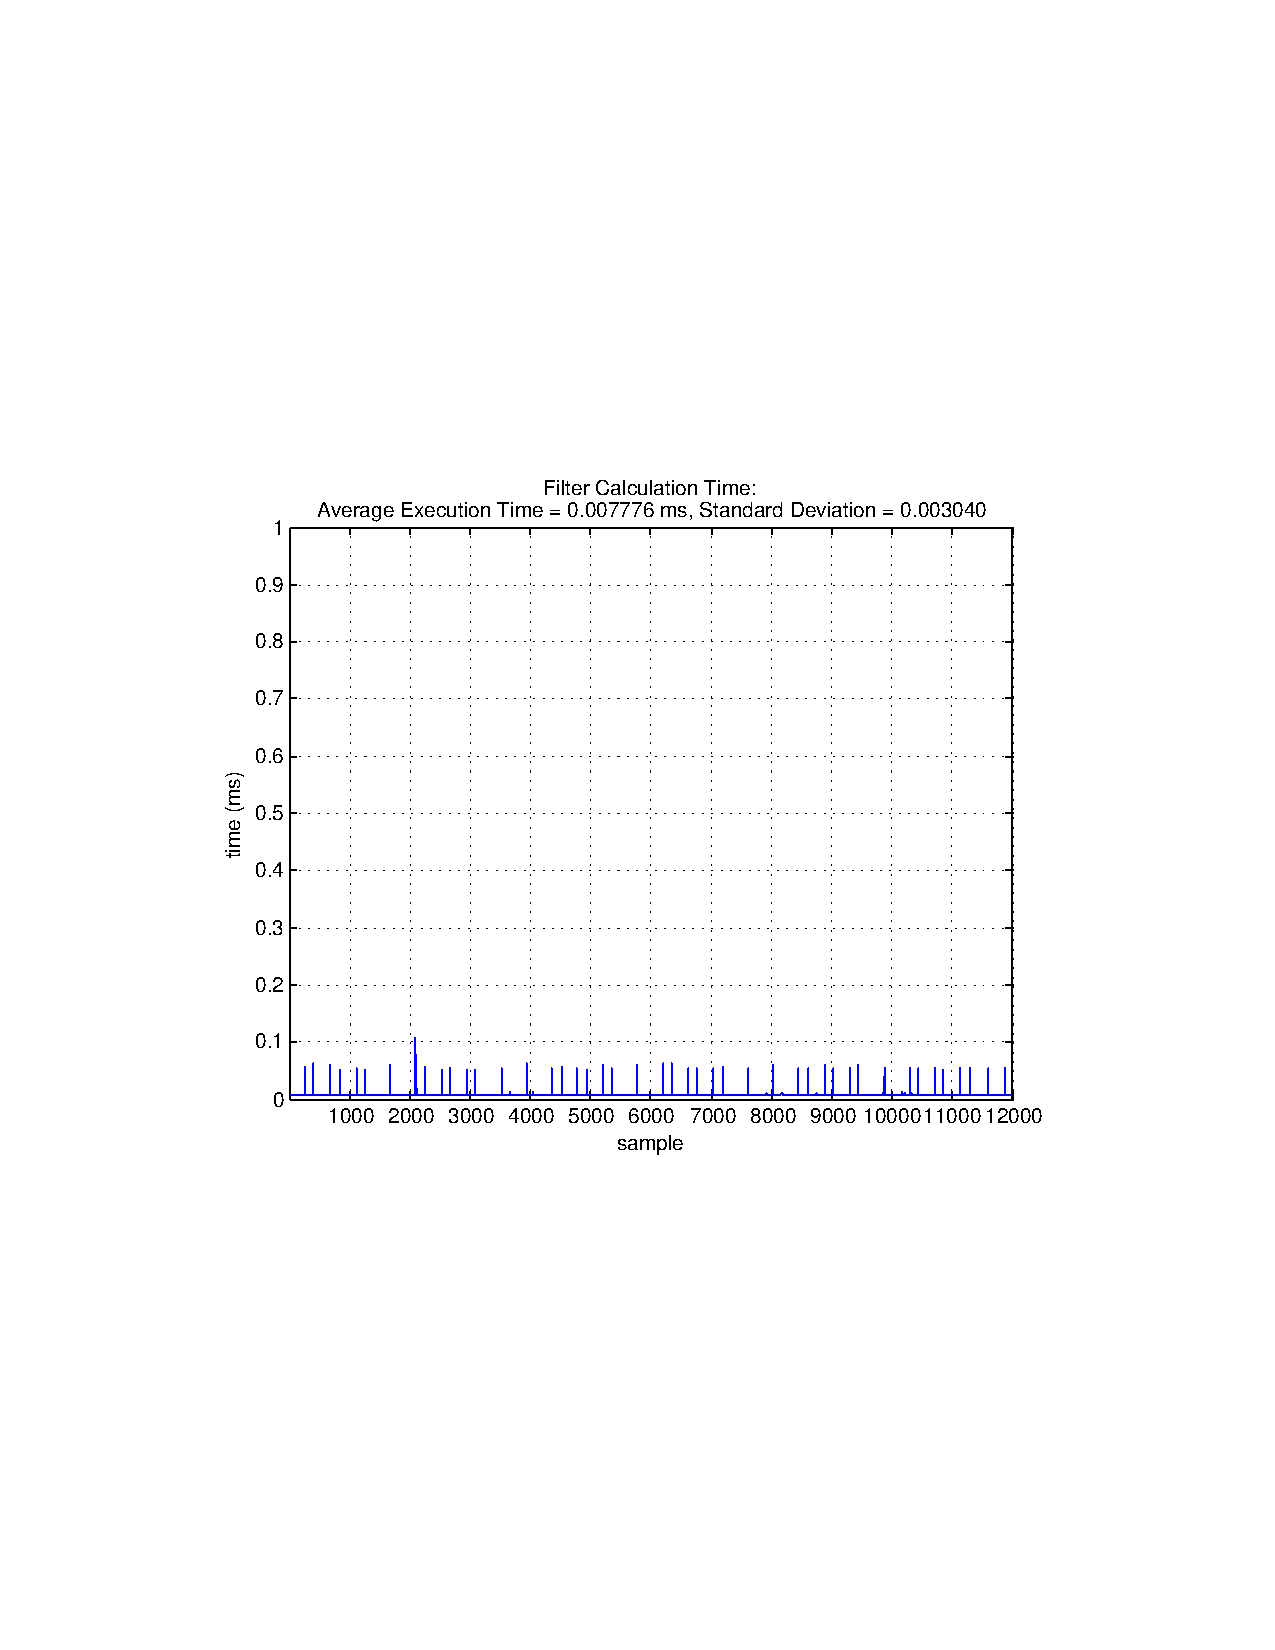
\includegraphics[width=0.6\columnwidth]{./timingData/filter.pdf}
  \caption{The amount of time it takes to process the built in filter.  In this case each sample has a time step of $0.005~sec$}
  \label{fig:timing-filter}
\end{figure}




\begin{figure}[thpb]
  \centering
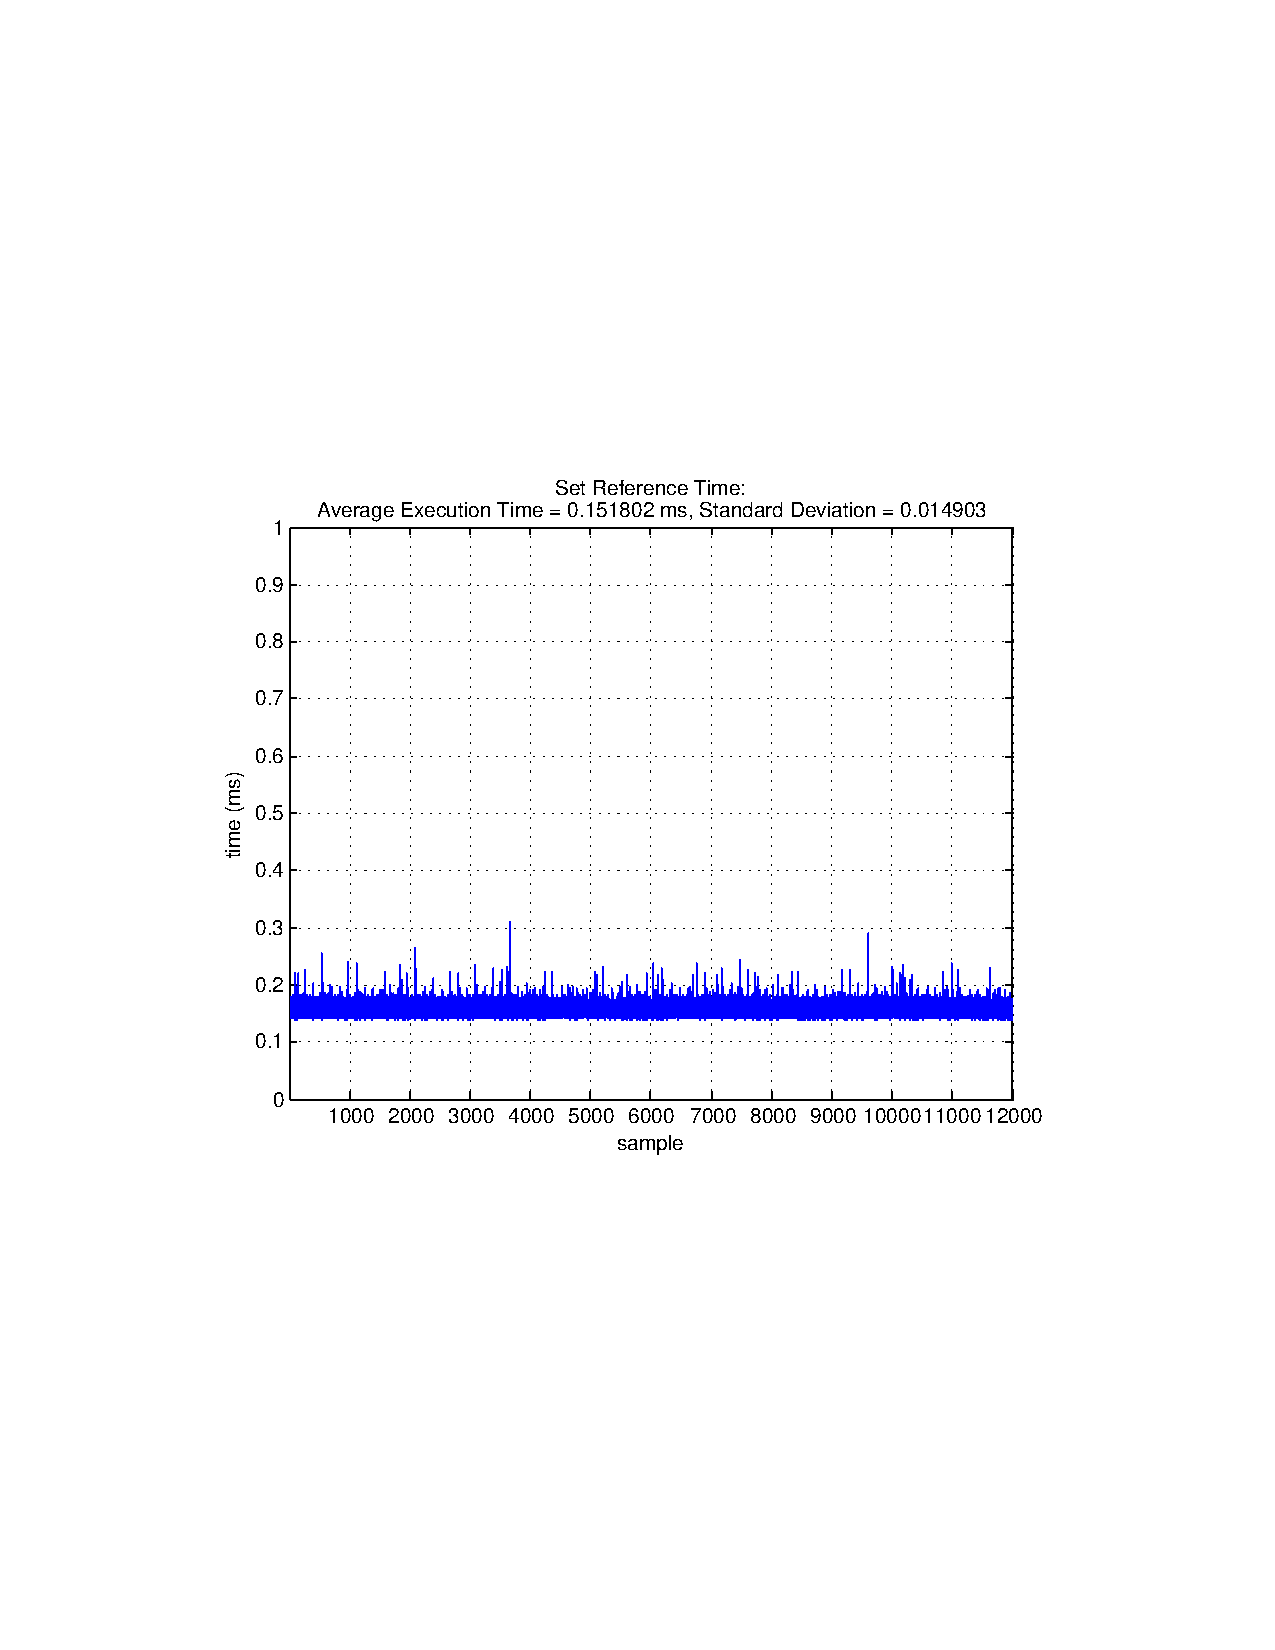
\includegraphics[width=0.6\columnwidth]{./timingData/setRef.pdf}
  \caption{The amount of time it takes to set the reference on the actuators via setting the data in the CAN bus buffer.  In this case each sample has a time step of $0.005~sec$}
  \label{fig:timing-setRef}
\end{figure}

\begin{figure}[thpb]
  \centering
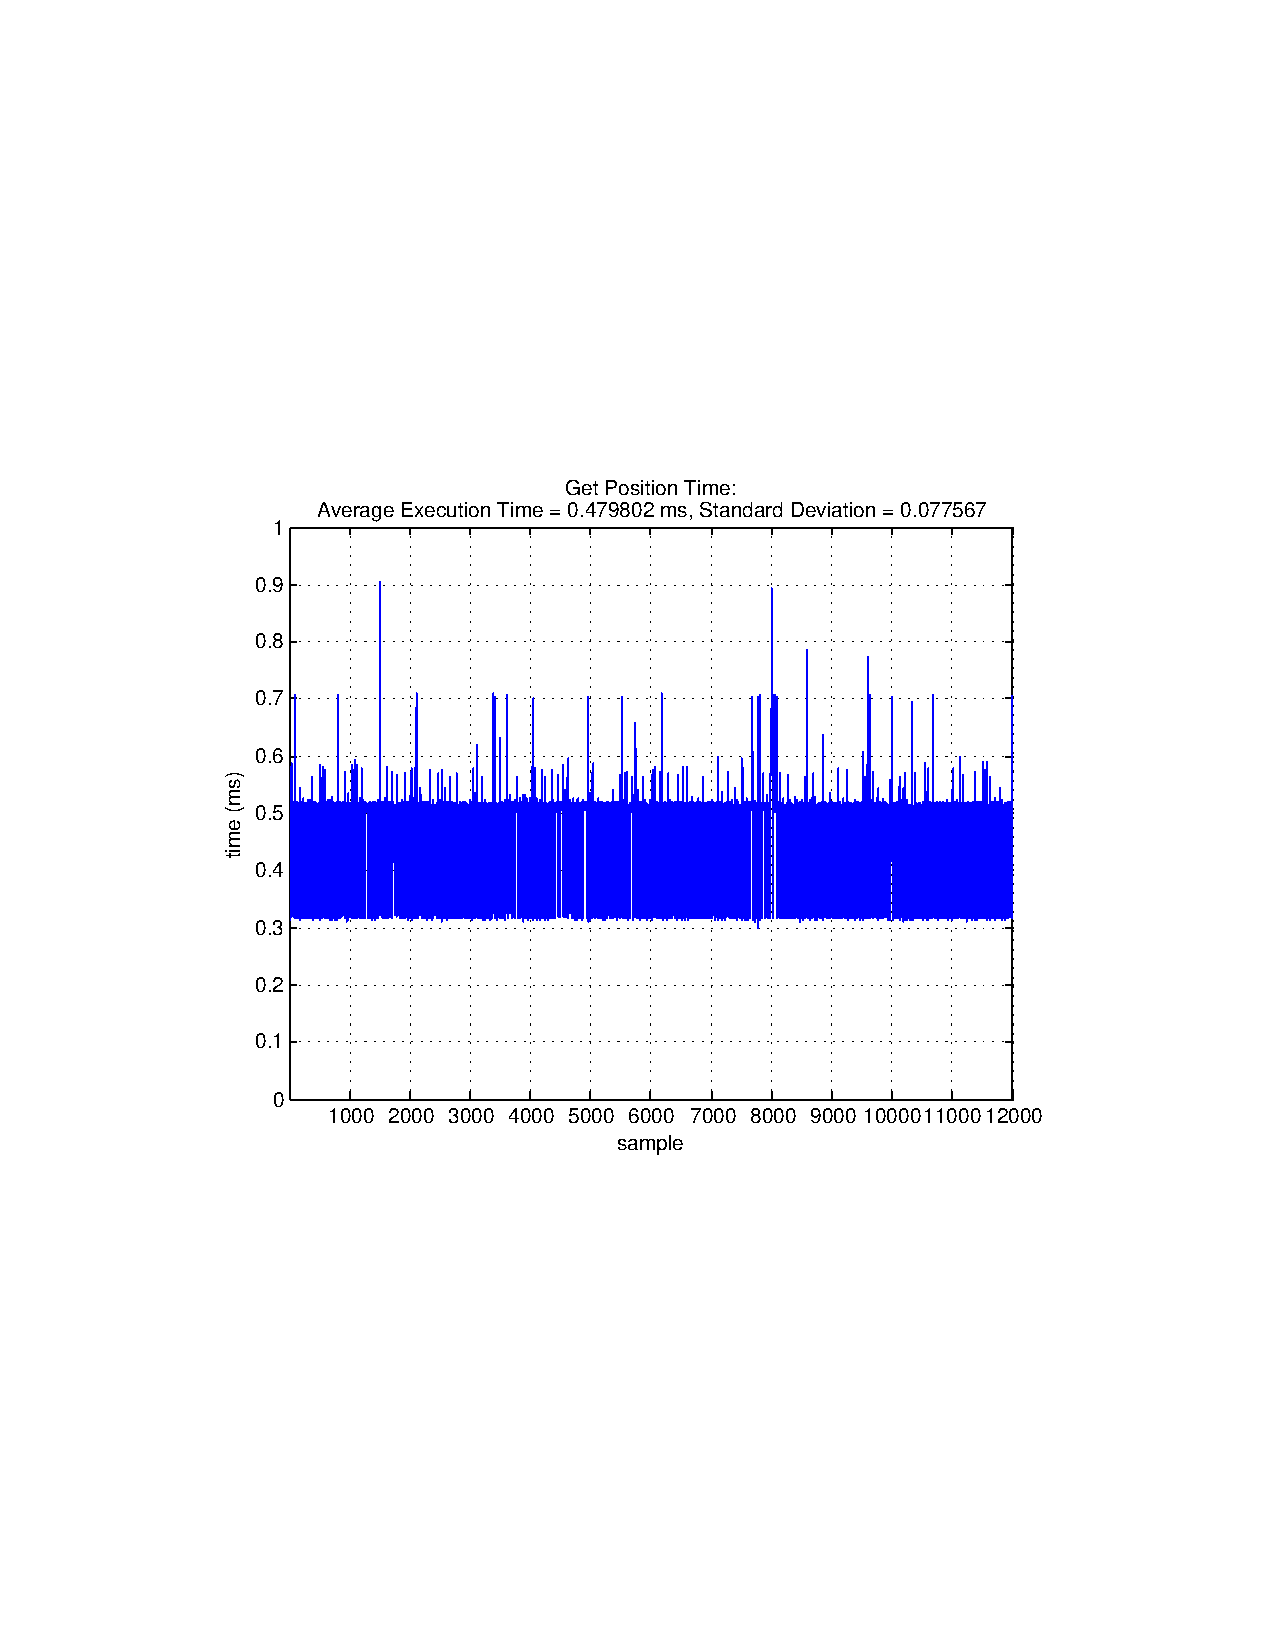
\includegraphics[width=0.6\columnwidth]{./timingData/getPos.pdf}
  \caption{The amount of time it takes to request and get the actual position from the actuators.  In this case each sample has a time step of $0.005~sec$}
  \label{fig:timing-getPos}
\end{figure}

\begin{figure}[thpb]
  \centering
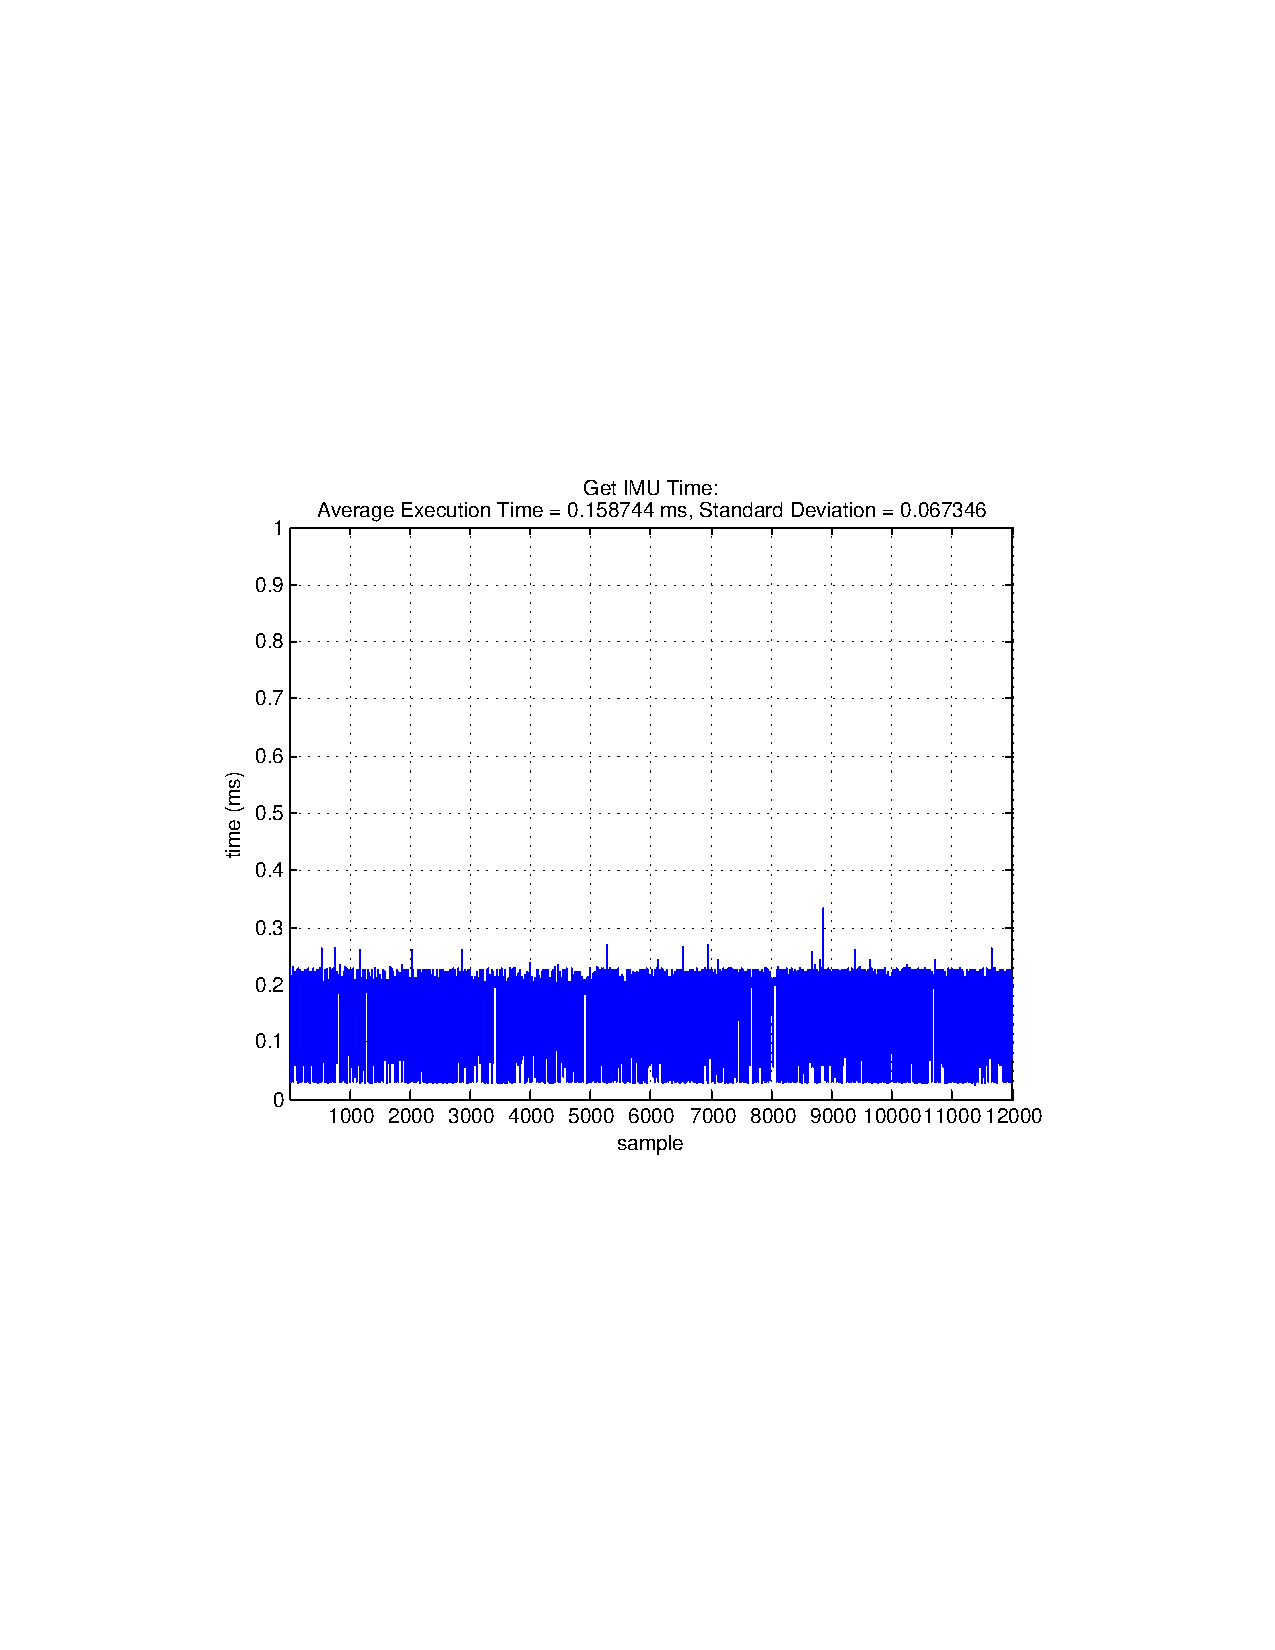
\includegraphics[width=0.6\columnwidth]{./timingData/getImu.pdf}
  \caption{The amount of time it takes to request and get the IMU data.  In this case each sample has a time step of $0.005~sec$}
  \label{fig:timing-imu}
\end{figure}


\begin{figure}[thpb]
  \centering
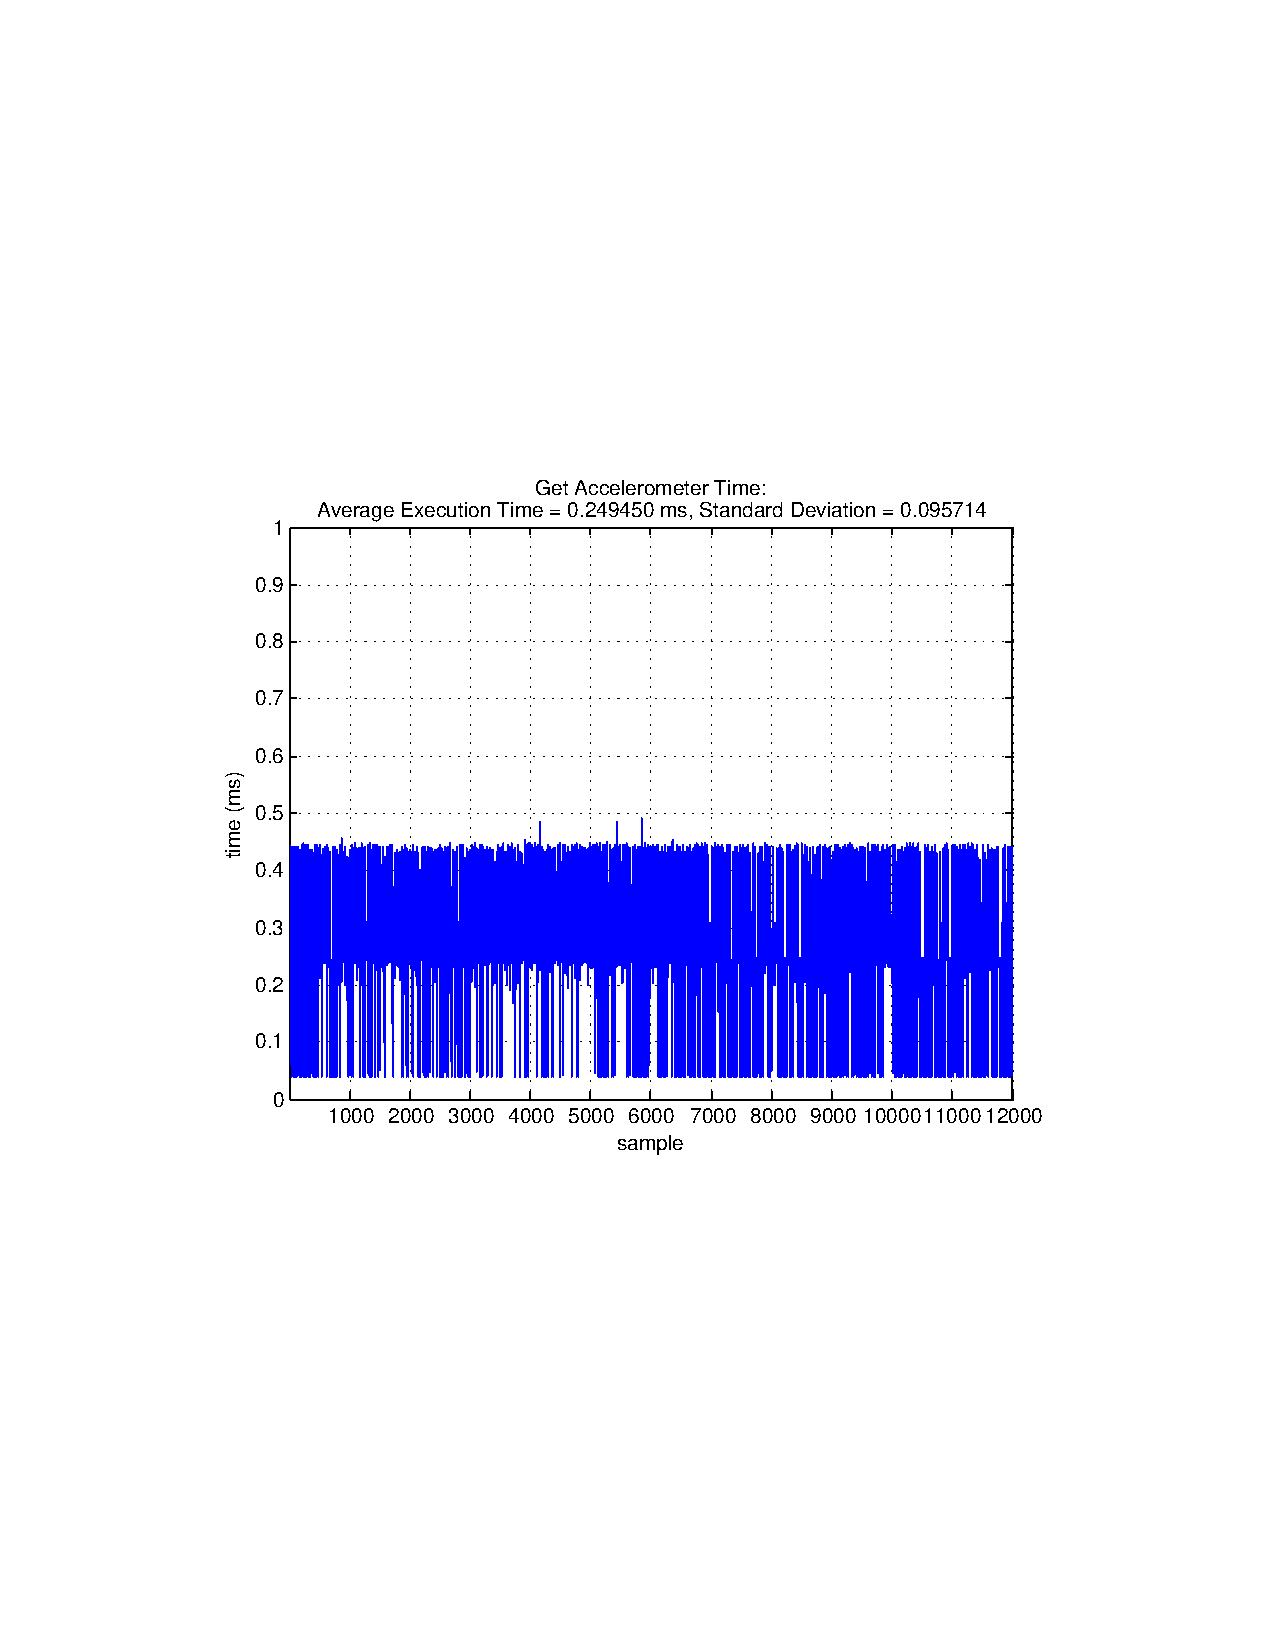
\includegraphics[width=0.6\columnwidth]{./timingData/getAcc.pdf}
  \caption{The amount of time it takes to request and get the accelerometers data.  In this case each sample has a time step of $0.005~sec$}
  \label{fig:timing-acc}
\end{figure}



\begin{figure}[thpb]
  \centering
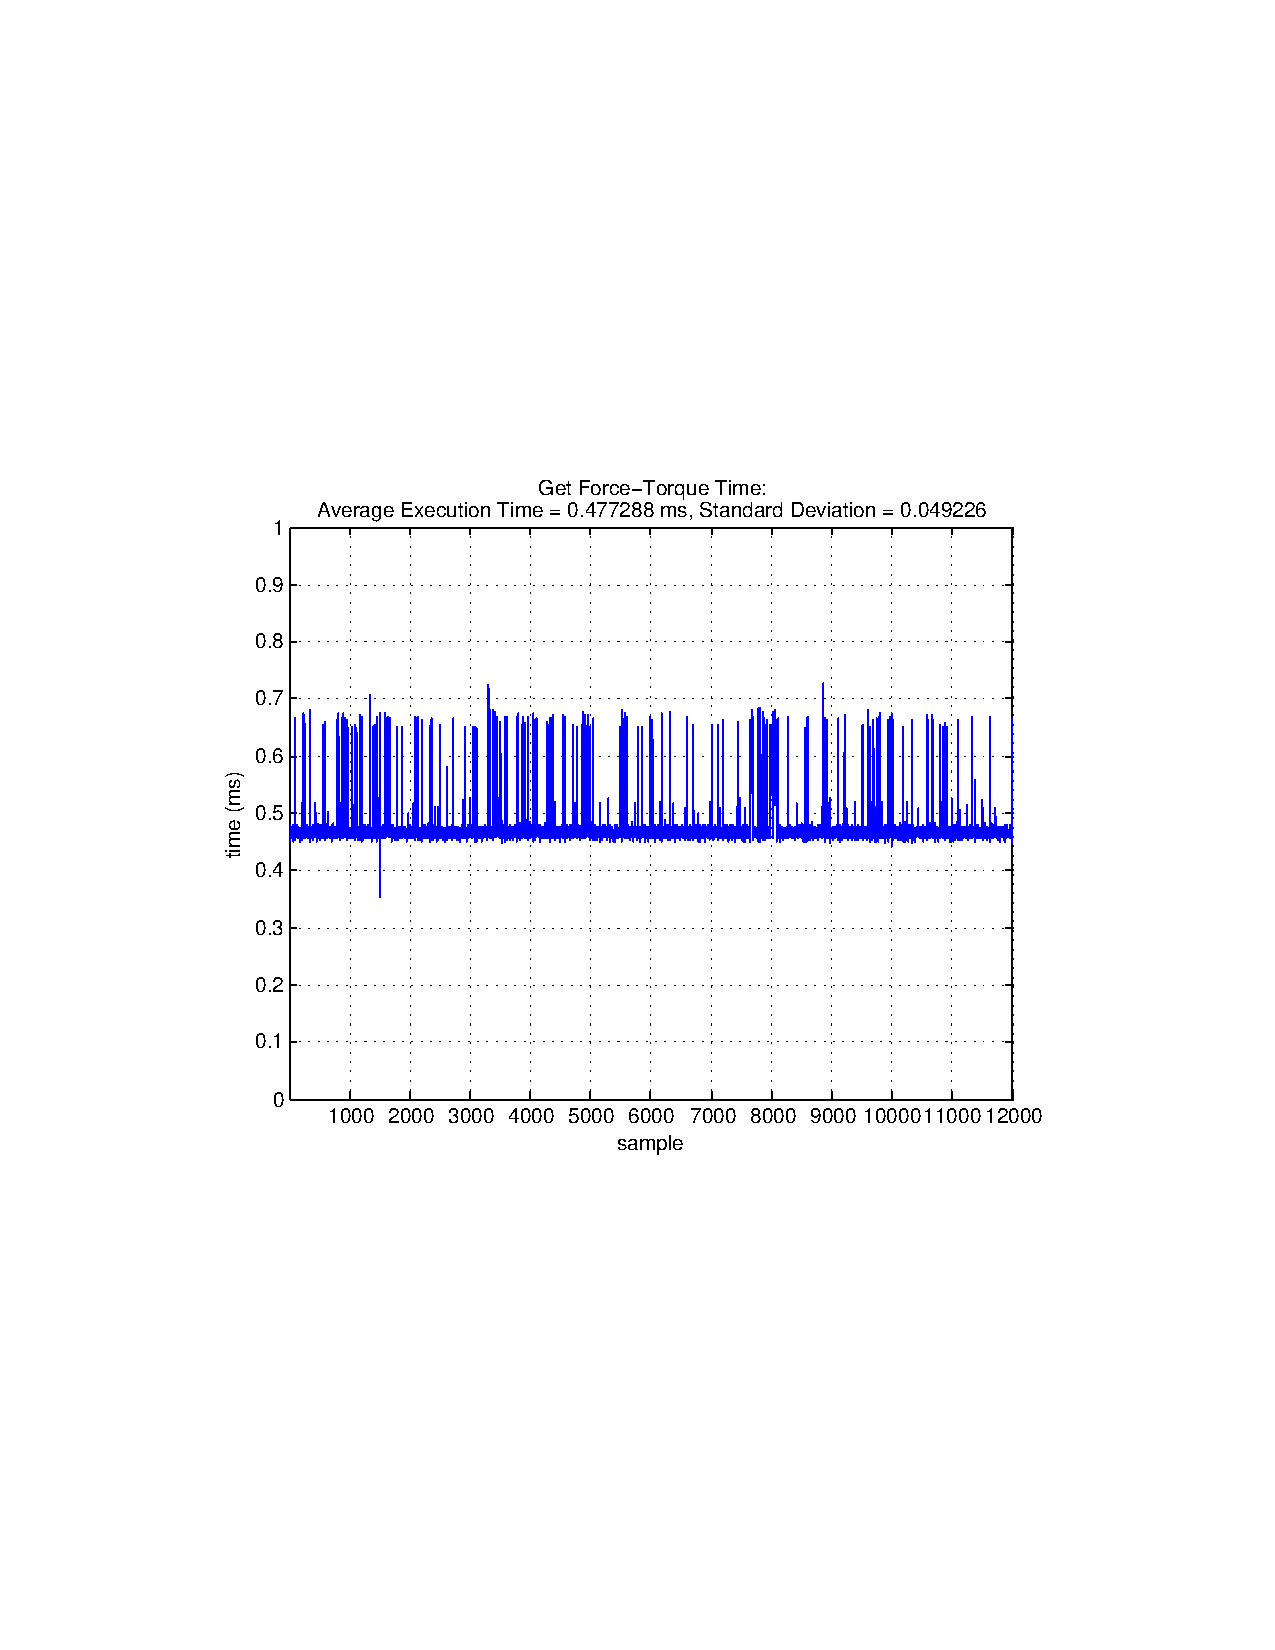
\includegraphics[width=0.6\columnwidth]{./timingData/getFt.pdf}
  \caption{The amount of time it takes to request and get the force-torque sensors.  In this case each sample has a time step of $0.005~sec$}
  \label{fig:timing-ft}
\end{figure}


\begin{figure}[thpb]
  \centering
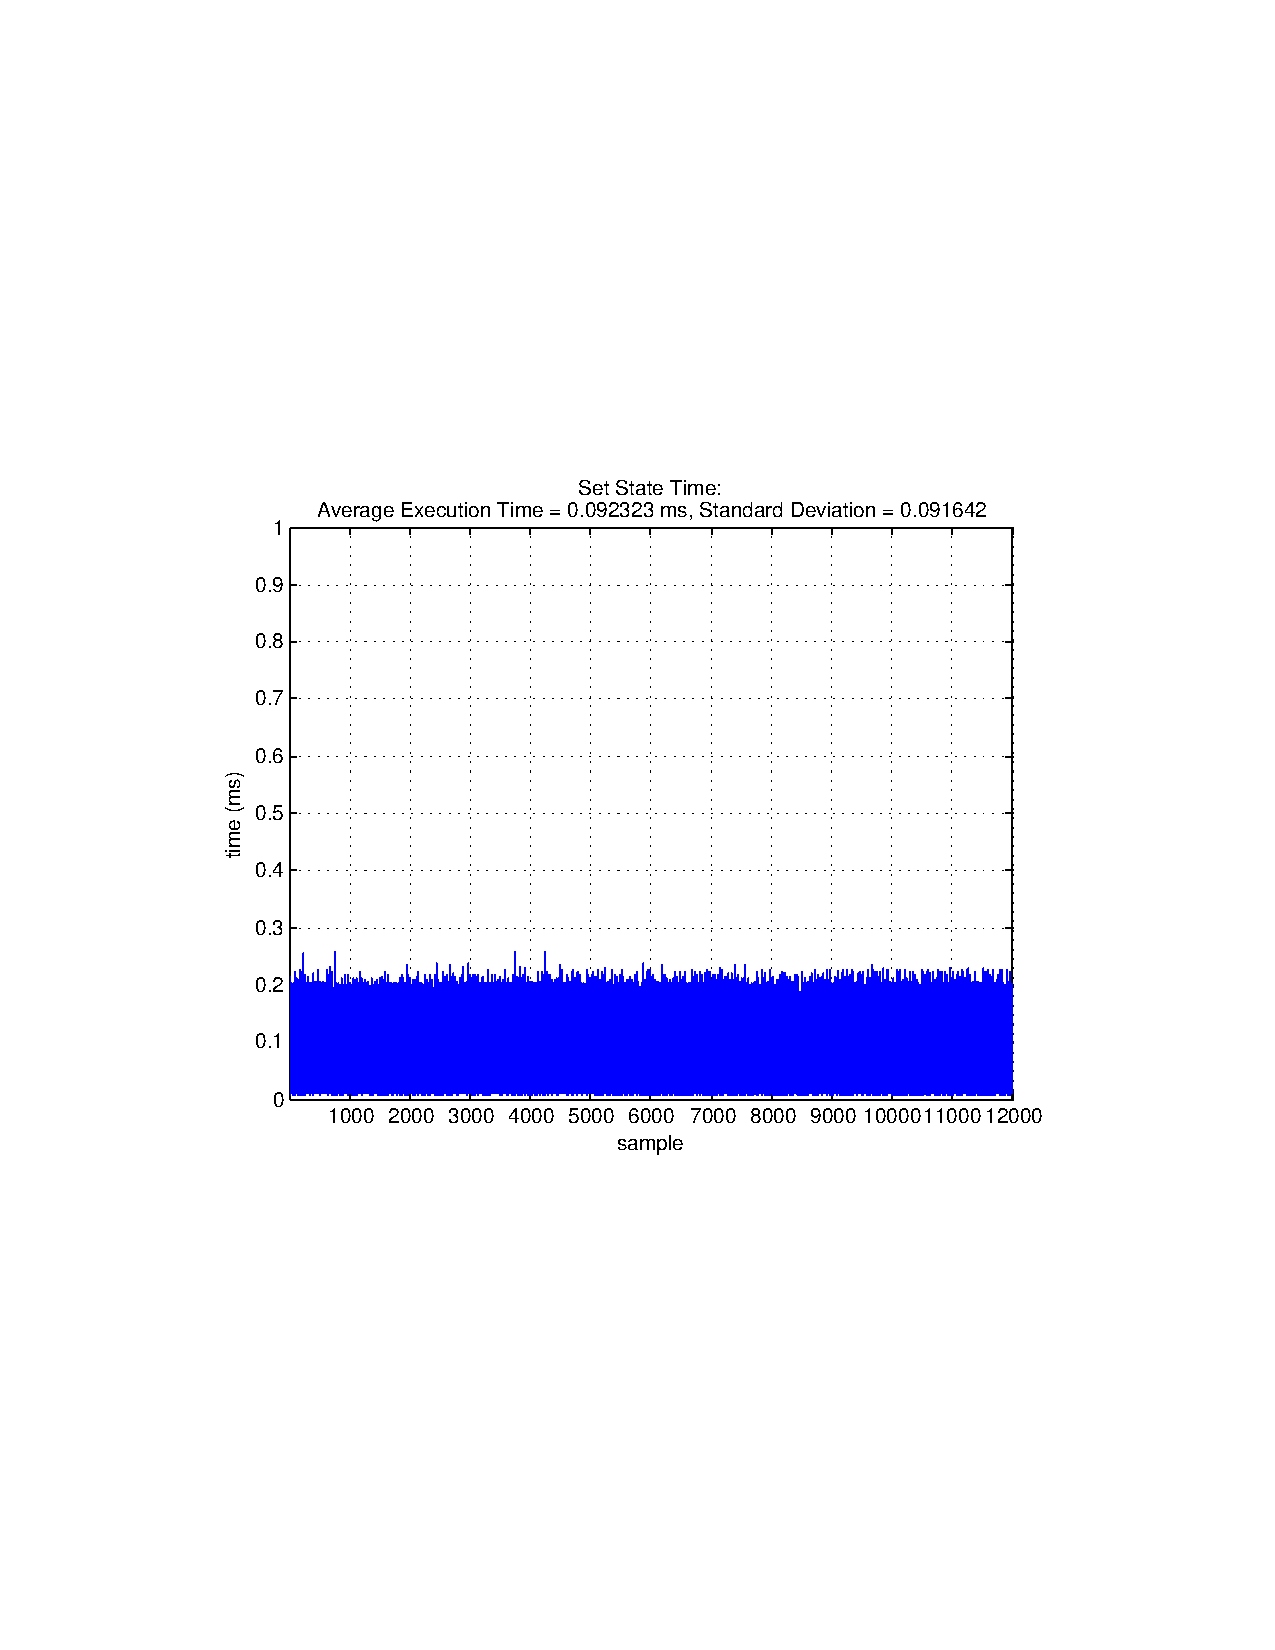
\includegraphics[width=0.6\columnwidth]{./timingData/setState.pdf}
  \caption{The amount of time it takes to set the state data on the feedback channel.  In this case each sample has a time step of $0.005~sec$}
  \label{fig:timing-setstate}
\end{figure}




Assuming no CAN delays Hubo-Ach can run at $1900~khz$.
With the current configuration of a 2 channel CAN bus it is restricted to below $237~hz$.
With a 4 channel CAN configuration it can be increased to $469~hz$.
With an 8 channel CAN configuration it can be increased to $1063~hz$.






























\section{CPU Usage}
	The CPU usage was analized while the Hubo-Ach controller was being used in the following states:
\begin{multicols}{2}
\begin{itemize}
\item Idle
\item Under open-loop control
\item Reading the sensors
\item Under closed-loop control
\end{itemize}
\end{multicols}

Fig.~\ref{fig:timing-getTrigger} shows the result of this test.
The results confirm that the CPU utilization stays within 0.3\% when idle and under closed loop control.
This means that the CPU utilization of Hubo-Ach is independent of the external control method.
Thus it will not add more to the CPU load under complex control schemes then under simple ones.
This makes it easy to model Hubo-Ach in when adding it to a CPU usage budget.


\begin{figure}[thpb]
  \centering
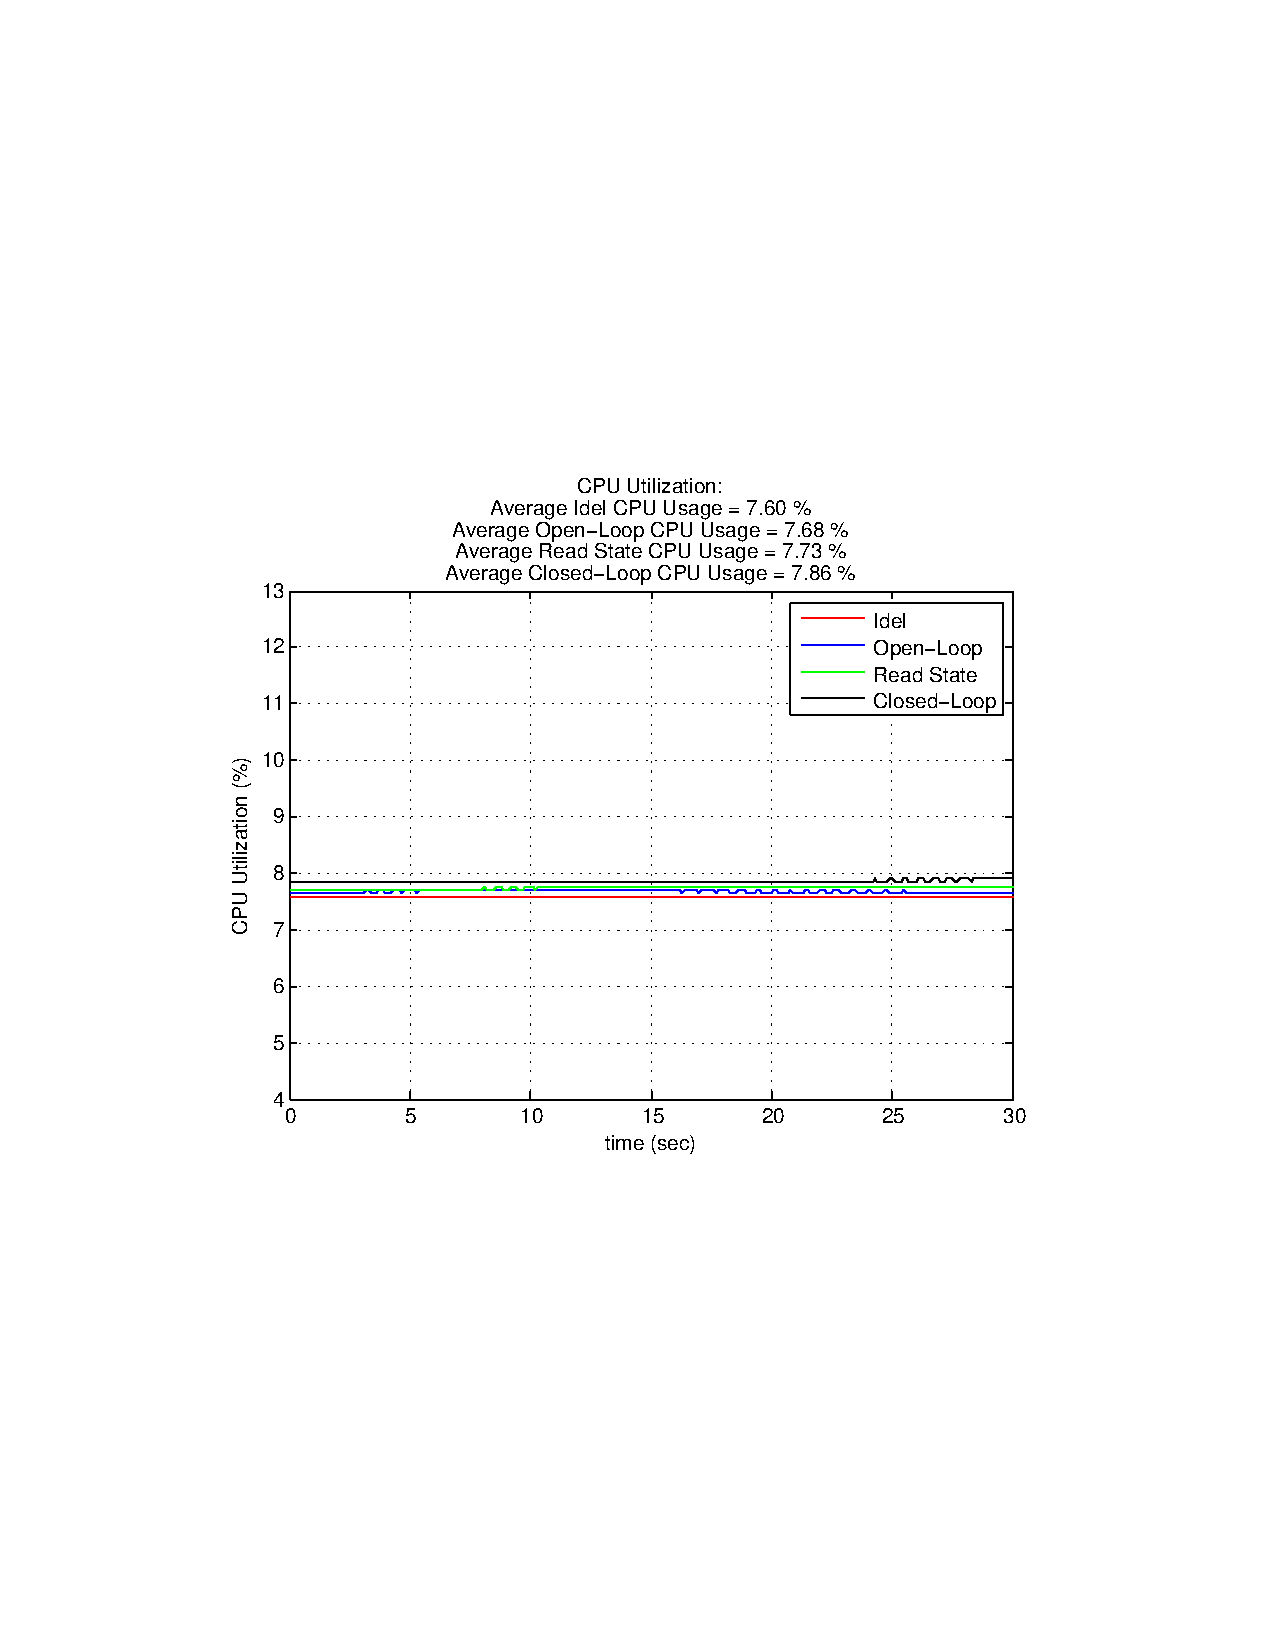
\includegraphics[width=0.6\columnwidth]{./timingData/cpu.pdf}
  \caption{CPU utilization for the Hubo-Ach process when 1) idle, 2) under open-loop control, 3) reading the sensors, and 4) under closed-loop control.  
It is important to note that the cpu utilization stays within 0.3\% when idle and under closed loop control.
This means that the CPU utilization of Hubo-Ach is independent of the external control method.
Thus it will not add more to the CPU load under complex control schemes then under simple ones.}
  \label{fig:timing-getTrigger}
\end{figure}

\section{Verification Experiments}\label{sec:simpleExamples}
This section contains step by step verification examples showing the controller for high DOF complex system functions properly with the hubo system.
All controllers are implemented using the multiple processes approach and includes all latencies found in Section~\ref{sec:timing}.

	\subsection{Joint Space Step Response}\label{sec:singlejointStep}
		This section shows the experimental and expected results of controlling a single joint via the Hubo-Ach system.
In this example the right shoulder pitch (RSP) is given a step input from 0.0 $rad$ to 0.4 $rad$.
The reference position $\theta_r$ is begin recorded as well as the actuator setpoint $\theta_c$ and the actual position of the joint $\theta_a$.
These definitions are also available in Table~\ref{table:recorded}

\begin{table}
\centering
\caption{States being recorded for the single joint step response test}
\begin{tabular}{l || c | c | c | c}
Signal      & Symbol     & Definition                    & Source      & Units \\
\hline
\hline
FeedForward & $\theta_r$ & Desired reference on the      & Hubo-Ach   & $rad$ \\
            &            & Hubo-Ach FeedForward Channel  &            &       \\
\hline
FeedForward & $\theta_c$ & Reference set to the actuator & Hubo-Ach   & $rad$ \\
\hline
Feedback    & $\theta_a$ & Actual position of joint as   & JMC        & $rad$ \\
            &            & measured from the encoders    &            &       \\
\hline
\end{tabular}
\label{table:recorded}
\end{table}



\begin{figure}[thpb]
  \centering
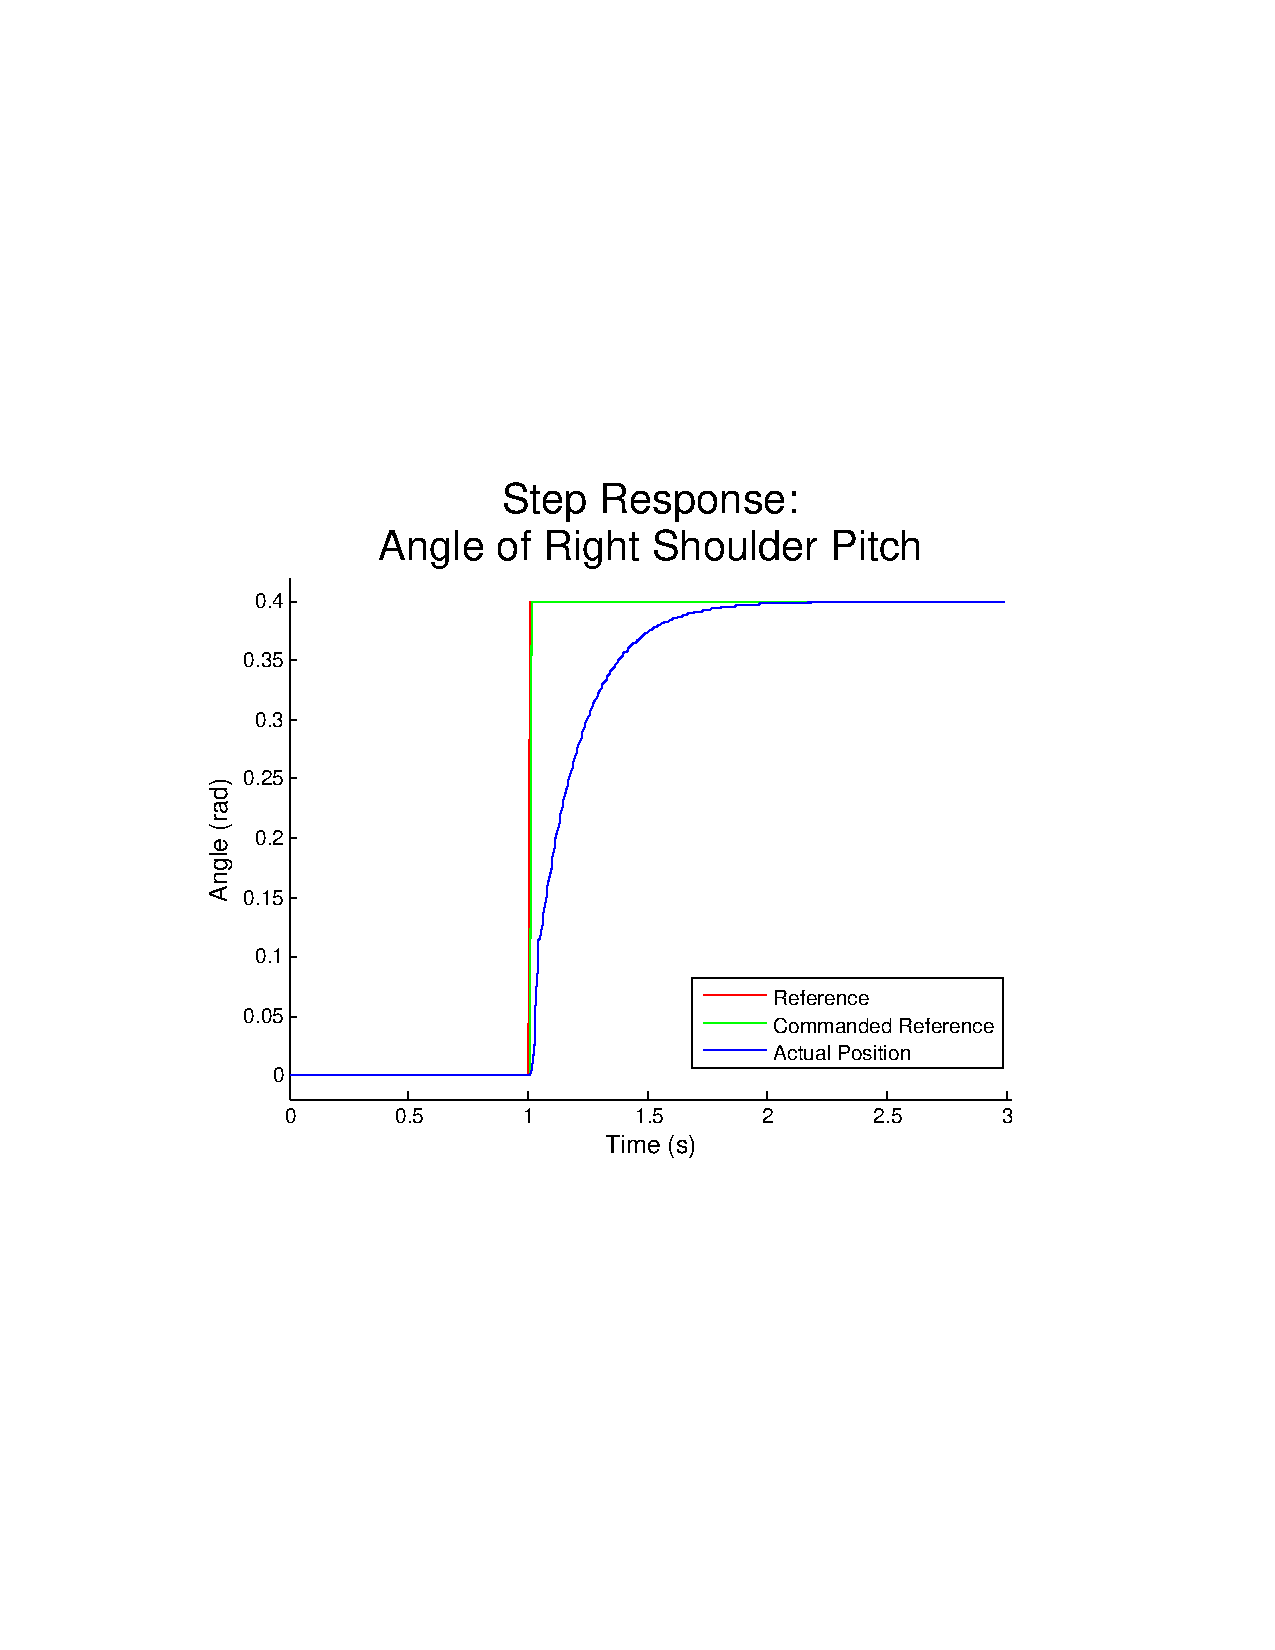
\includegraphics[width=0.8\columnwidth]{./examples/pix/RSP-Zp4-step-step-crop.pdf}
  \caption{The commanded reference plotted against the actual reference recorded via Hubo-Ach and ground truth via CAN analyzing utilities.  In this plot the commanded reference is not automatically filtered by Hubo-Ach.  The commanded joint is the right shoulder pitch.}
  \label{fig:singleJointStep}
\end{figure}

Fig.~\ref{fig:singleJointStep} shows the results when a step input is applied and Hubo-Ach is in \textit{HUBO\_REF\_MODE\_REF\_FILTER} also know as pass-through mode.
This sets the what the desired reference on the \textbf{FeedForward} Hubo-Ach channel to the actuator's reference, i.e.:

\begin{equation}\label{eq:refrefmode}
 \theta_c(N) = \theta_r(N)
\end{equation}

Fig.~\ref{fig:hubo-ach-feedforward} shows the block diagram of the control setup.

\begin{figure}
\centering
\begin{tikzpicture}[->,>=stealth',shorten >=1pt,auto,node distance=5cm,
  thick,main node/.style={fill=white!20,draw,font=\sffamily\Large\bfseries}]


  \node[main node] (ref) {Reference};
  \node[main node] (hubo-ach) [right of=ref] {Hubo-Ach};
  \node[main node] (hubo) [right of=hubo-ach] {Hubo};




  \path[<->,dashed, every node/.style={font=\sffamily\small}]
    (hubo) edge node [above] {CAN} (hubo-ach);

  \path[->,every node/.style={font=\sffamily\small}]
    (ref) edge node [above] {$\theta_r$} (hubo-ach);


\end{tikzpicture}
\caption{Reference $\theta_r$ being applied to Hubo via Hubo-Ach.  $\theta_r$ is set on the \textbf{FeedForward} channel, Hubo-Ach reads it then commands Hubo at the rising edge of the next cycle.}
\label{fig:hubo-ach-feedforward}
\end{figure}






As seen in Fig~\ref{fig:singleJointStep} $\theta_c$ tracks $\theta_r$ perfectly. As expected $\theta_a$ lags by a minimum of 1 time step $T$.  
This is the time it takes between sending $\theta_c$ to the actuator over the CAN bus plus the time it takes in receiving the feedback from the encoder of the motor over CAN.
The remainder of the lag is due to the rise time of the actuator.
This is different for each joint.
Because all major joints are high-gain PID the rise-time and overshoot is very small which makes the robot very stiff.
The total lag between commanding the joint on the \textbf{FeedForward} channel and the response of the actuator is:

\begin{equation}
t_{lag} = t_{filter} + t_{rise}
\end{equation}



	\subsection{Joint Space Step Response with Position Filtering}\label{sec:singlejointFilter}
		Giving a step input to a high-gain PID position controlled actuator can cause an over current fault, burn out motor drivers, strip gears due to the \textit{jerk} etc.  
To reduce this effect Hubo-Ach has multiple modes of on-board filtering.
These modes are:
\begin{itemize}
\item Reference Input Filtering
\item Compliance Amplification 
\end{itemize}

This section talks about \textit{reference input filtering} as a method to apply a step input each joint in joint space and limit the jerk.
It is important to note that the obvious answer is to reduce the PID gains to make the robot \textit{more complaint} however the goal of this work is to make a fully functional system that does not require modification of the robot.
In this case the PID gains are set by the motor drivers and that is considered to be a part of the robot.
In future firmware updates of the motor drivers we will have the ability to change PID gains on the fly.

\textit{reference input filtering} uses the history of the previous $\theta_c$ sent to the given actuator.  The current commanded actuator position $\theta_c(N)$ is given by:

\begin{equation}\label{eq:reffiltermode}
\theta_c(N) = \frac{\theta_c(N-1)\cdot\left(L-1\right) + \theta_r(N)}{L}
\end{equation}

Where $L$ is an integer that represents the length of the filter and $L\geq1$.  
If $L=1$ then Equation~\ref{eq:reffiltermode} becomes Equation~\ref{eq:refrefmode}.



Fig.~\ref{fig:singleJointStepFiltered} shows the commanded reference plotted again the actual reference using the filtered mode defined in Equation~\ref{eq:reffiltermode}.
Fig.~\ref{fig:singleJointStepFilteredLtest} shows the $\theta_r$ plotted against $\theta_c$ and $\theta_a$ for different values of $L$.
It is easy to see that as $L$ increases the $t_{rise}$ also increases and the \textit{jerk} is reduced.


\begin{figure}[thpb]
  \centering
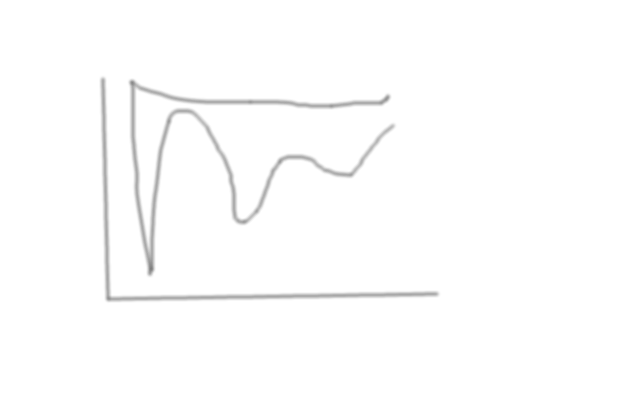
\includegraphics[width=0.8\columnwidth]{./pix/tmp.png}
  \caption{The commanded reference plotted against the actual reference recorded via Hubo-Ach and ground truth via CAN analyzing utilities.  In this plot the commanded reference is automatically filtered by Hubo-Ach.}
  \label{fig:singleJointStepFiltered}
\end{figure}

\begin{figure}[thpb]
  \centering
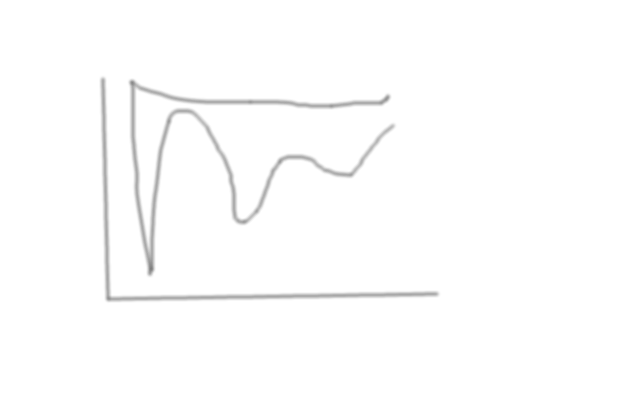
\includegraphics[width=0.8\columnwidth]{./pix/tmp.png}
  \caption{$\theta_r$ plotted against $\theta_c$ and $\theta_a$ recorded via Hubo-Ach with values for $L$ ranging from 1 to 200.}
  \label{fig:singleJointStepFilteredLtest}
\end{figure}

This method is a feed-forward method that assumes that the position you set the actuator to is the actual position of the actuator.

	\subsection{Compliance Amplification}\label{sec:singlejointRefComplience}
		Compliance amplification takes advandage of the internal compliance of the joints and amplifies that by feeding back the PID error $\theta_e$.
Like the Equation~\ref{eq:refrefmode} we have no past information about the set reference and we have only the compiliance given by the joints.
If we think about $\theta_e$ and what effects it we can use it to add compliance to our system.
It is important to note that because the Hubo is a high-gain PID position controlled device with an intergral gain $K_i$ set to zero the steady state error of the joint (the PID error $\theta_e$) is proportional to the moment applied to the joint.
If we combine the reference $\theta_r$ and $\theta_e$ multiplied by a compliance gain $K_c$ we are able to add/amplify the compliance to the system.

\begin{equation}
\theta_c(N) = K_c\theta_e(N)+\theta_r(N)
\end{equation}

It is important to note that $K_c \leq 1$ or the system will go unstable.
If $K_c=1$ then we have

\begin{equation}
\theta_c(N) = \theta_a(N)
\end{equation}

	\subsection{Joint Space Step Response with Feedback Filtering}\label{sec:singlejointEnc}
		Feedback filtering allows us to removes the requirement that we know the joint's current position.
Similar to Equation~\ref{eq:reffiltermode} this method sets $\theta_c$ based on a filter length $L$ and the current desired value $\theta_r$.
However instead of assuming that we know all past $\theta_r$ we use the actual position $\theta_a$.
This method add compliance in a similar way to that of Section~\ref{sec:singlejointRefComplience}.


\begin{equation}\label{eq:refencmode}
\theta_c(N) = \frac{\theta_a(N)\cdot\left(L-1\right) + \theta_r(N)}{L}
\end{equation}

This causes three major effects: 

\noindent \textbf{Effect 1:} The movement of the joint is guaranteed to be filtered even if the previous reference is unknown.

\noindent \textbf{Effect 2:} The steady state error of the feedback filtering method $\theta_e^{fbfilter}$ is greater than that of the PID error $\theta_e$ in the direction of the moment acting on the joint.

\begin{equation}
\theta_e^{fbfilter} > \theta_e
\end{equation}

\noindent \textbf{Effect 3:} The joint's compliance has increased due to the effect of the moment applied to the joint has on the steady state error.

\begin{figure}
\centering

\begin{tikzpicture}[->,>=stealth',shorten >=1pt,auto,node distance=5cm,
  thick,main node/.style={fill=white!20,draw,font=\sffamily\Large\bfseries}]


  \node[main node] (ref) {Reference};
  \node[main node] (filter) [right=3.0cm of ref] {Filter};
  \node[main node] (hubo-ach) [below=1.0cm of filter] {Hubo-Ach};
  \node[main node] (hubo) [right=3.0cm of hubo-ach] {Hubo};




  \path[<->,dashed, every node/.style={font=\sffamily\small}]
    (hubo) edge node [above] {CAN} (hubo-ach);

  \path[->,every node/.style={font=\sffamily\small}]
    (ref) edge node [above] {$\theta_d$} (filter);

  \path[->,every node/.style={font=\sffamily\small}]
    (hubo-ach) edge node [left] {$\theta_r$} (filter);

  \path[->,every node/.style={font=\sffamily\small}]
    (filter) edge node [right] {$\theta_a$} (hubo-ach);


% look into this and add z^-1

\path [every node/.style={draw,minimum width=3cm, minimum height=5cm]}]
  node (a) at (0,0) {}
  [xshift=7cm]
  node (b) at (0,0) {}
  [xshift=7cm]
  node (c) at (0,0) {};

%\begin{scope}[->,>=latex]
%    \foreach \i in {-2,...,2}{% 
%      \draw[->] ([yshift=\i * 0.8 cm]a.east) -- ([yshift=\i * 0.8 cm]b.west) ;}

%    \foreach \i in {1,2}{% 
%      \draw[->] ([yshift=\i * 0.8 cm]a.east) to [out=50,in=130] ([yshift=\i * 0.8 cm]c.west) ;} 

%    \foreach \i in {-1,-2}{% 
%      \draw[->] ([yshift=\i * 0.8 cm]a.east) to [out=-50,in=-130] ([yshift=\i * 0.8 cm]c.west) ;}
%\end{scope}


\end{tikzpicture}
\caption{Desired reference $\theta_d$ being filtered before applied to Hubo via Hubo-Ach.  $\theta_d$ is sent through a filter that reduces the \textit{jerk} on the actuator then the new reference $\theta_r$ is set on the \textbf{FeedForward} channel, Hubo-Ach reads it then commands Hubo at the rising edge of the next cycle.}
\label{fig:hubo-ach-feedforward}
\end{figure}



Fig.~\ref{fig:singleJointStepFilteredFeedback} shows $\theta_r$ plotted against $\theta_c$ and $\theta_a$.  
$\theta_a$ not only lags behind $\theta_c$ but it also has a greater steady state error.
Fig.~\ref{fig:singleJointStepFilteredFeedbackMoment} shows how the steady state error $\theta_e^{fbfilter}$ increases with an applied moment.
This is where we get our compliance.

\begin{figure}[thpb]
  \centering
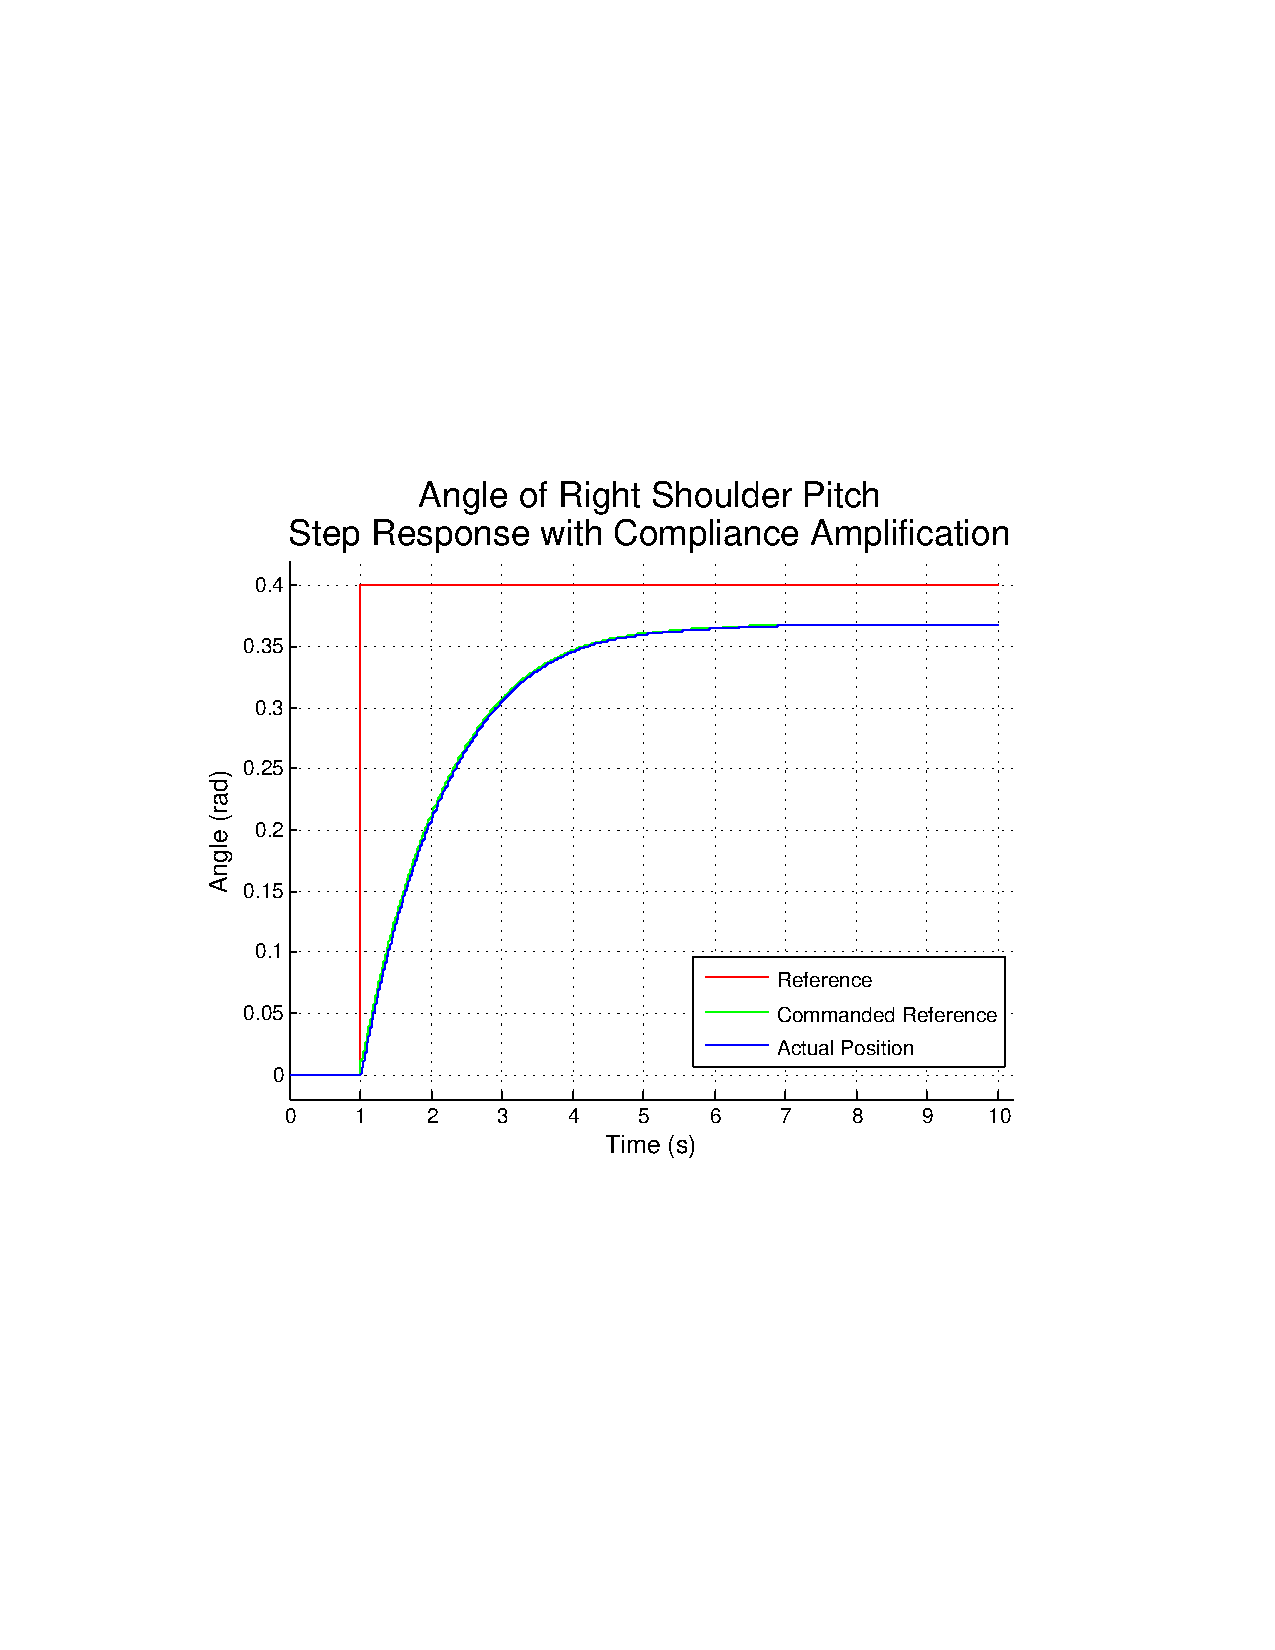
\includegraphics[width=0.8\columnwidth]{./examples/pix/RSP-Zp4-step-enc-real-crop.pdf}
  \caption{$\theta_r$ plotted against $\theta_c$ and $\theta_a$ recorded via Hubo-Ach using the feedback filtering method.}
  \label{fig:singleJointStepFilteredFeedback}
\end{figure}

\begin{figure}[thpb]
  \centering
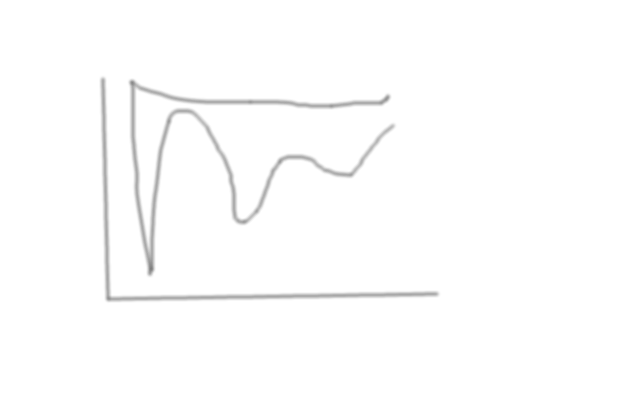
\includegraphics[width=0.8\columnwidth]{./pix/tmp.png}
  \caption{$\theta_r$ plotted against $\theta_c$ and $\theta_a$ recorded via Hubo-Ach using the feedback filtering method with different moments applied to the joint.  You will note that as the moment increases so does $\theta_e^{fbfilter}$. }
  \label{fig:singleJointStepFilteredFeedbackMoment}
\end{figure}


\section{Kinimatics}\label{sec:hubo-ach-kinimatics}
Kinematic planning is a key focus of the Hubo-Ach controller.
This section provides two published examples of the Hubo-Ach controller being used for inverse kinematics and control.
Section~\ref{sec:valve} shows the work of Lofaro et. al. \cite{lofaroTePRA2013Valve} using Constrained Bi-Directional Rapidly-exploring Random Tree (CBiRRT) to provide a statically stable joint space trajectory allowing the robot to turn a valve.
Section~\ref{sec:6dofik} shows the work of Lofaro et. al. \cite{lofaroTePRA2013HuboAch} using traditional 6 DOF forward and inverse kinematic techniques to provide an analytical IK solution to each of the 6 DOF end effectors.
The additional use of on-line trapezoidal velocity profiling methods in Section~\ref{sec:trap} allow for the creation of a real-time IK controller based in Hubo-Ach.


\subsection{Valve Turning}\label{sec:valve}
	\begin{figure}[thpb]
  \centering
  %\begin{tikzpicture}
    %\clip [rounded corners=1em] (0,0) rectangle coordinate (centerpoint) (5,7.5cm);
%    \node[minimum width=\linewidth,minimum height=174pt,draw=black,rounded corners=1em,fill=bgcolor,draw=black]
%    {};
%    \node[name=img] {
      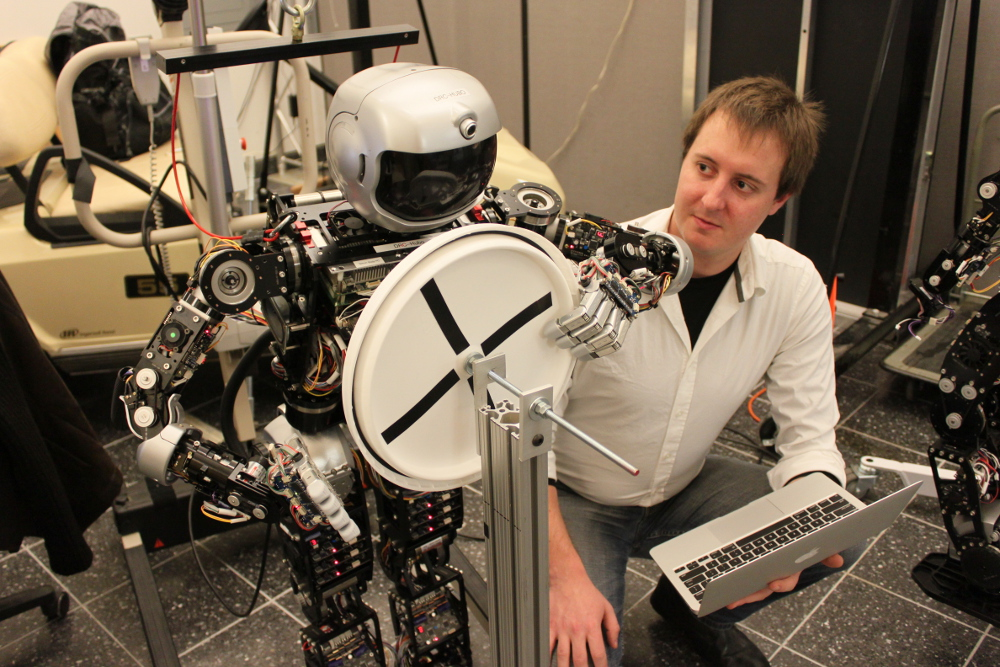
\includegraphics[width=0.93\columnwidth]{./pix/IMG_9107-small.jpg}
      
\includegraphics{./qrcode/qrcode-valve.png}\\
      Video: http://danlofaro.com/phd/valve/
%    };
%    \draw [bgcolor, rounded corners=1em, line width=1em,inner sep=0pt]
%    (img.north west) --
%    (img.north east) --
%    (img.south east) --
%    (img.south west) -- cycle
%    ;
%  \end{tikzpicture}
\caption{Hubo (left) turning a valve via Hubo-Ach alongside Daniel
  M. Lofaro (right).  Valve turning developed in conjunction with
  Dmitry Berenson at WPI for the DARPA Robotics Challenge.}
  \label{fig:valve}
\end{figure}



\section{Six Degree of Freedom Inverse Kinematic Implementation Example}\label{sec:6dofik}
This section shows how we calculate the inverse kinematics (IK) for the Hubo's right arm and how we use that calculation in conjunction with Section~\ref{sec:simpleExamples}.  The result is the ability to command the end effector (EEF)

In order to control the Hubo's upper body manipulators in work space as opposed to joint space both forward and inverse kinematics are required, (FK) and (IK) respectively.
In order to find a proper solution the joint limits, singularities and feasible workspace (no-self collisions) must be accounted for.

The kinematic structure of the right and left arm of the Hubo are identical with the caveat that the work space offset is mirrored over the z-axis.
This means that they have the same Denavit–Hartenberg (DH) parameters.

\begin{table}
\centering
\caption{Denavit–Hartenberg for Hubo2+ upper body (arms) in standard format}
\begin{tabular}{|l | c|}
\hline
Link     & Length (m) \\
\hline
\hline
$l_{A1}$ & 0.215 \\
\hline
$l_{A2}$ & 0.179 \\
\hline
$l_{A3}$ & 0.182 \\
\hline
$l_{A4}$ & 0.121 \\
\hline
$l_{E}$ & 0.100 \\

\hline

\end{tabular}\label{table:DHupper}
\end{table}

\begin{figure}
\centering

\begin{tikzpicture}[->,>=stealth',shorten >=1pt,auto,node distance=5cm,
  thick,main node/.style={fill=white!20,draw,font=\sffamily\small\bfseries}]

  \node[main node] (ref) [text width=3cm] {End Effector Position};

  \node[main node] (ik) [right=2.0cm of ref] {6-DOF IK};
  \node[main node] (filter) [right=2.0cm of ik] {Filter};
  \node[main node] (hubo-ach) [below=1.0cm of filter] {Hubo-Ach};
  \node[main node] (hubo) [right=2.0cm of hubo-ach] {Hubo};



  \path[->, every node/.style={font=\sffamily\small}]
    (ref) edge node [above] {$(x,y,z)$} (ik)
    (ref) edge node [below] {$(\alpha,\beta,\gamma)$} (ik);
%  \path[->, every node/.style={font=\sffamily\small}]
%    (ref) edge node [below] {$(\alpha,\beta,\gamma)$} (ik);

 

  \path[->,every node/.style={font=\sffamily\small}]
    (ik) edge node [above] {$\overline{\theta_d}$} (filter);

 \draw[->] ([xshift=-0.5 cm]filter.south)  -- node [left] {$\overline{\theta_r}$} ([xshift=-0.5 cm]hubo-ach.north)  ;
 \draw[->] ([xshift=0.5 cm]hubo-ach.north) -- node [left] {$\overline{\theta_a}$} ([xshift=0.5 cm]filter.south)  ;

 \path[<->,dashed, every node/.style={font=\sffamily\small}]
    (hubo) edge node [above] {CAN} (hubo-ach);

%  \path[->,every node/.style={font=\sffamily\small}]
%    (hubo-ach) edge node [left] {$\theta_r$} (filter);

%  \path[->,every node/.style={font=\sffamily\small}]
%    (filter) edge node [right] {$\theta_a$} (hubo-ach);




% look into this and add z^-1

%\path [every node/.style={draw,minimum width=3cm, minimum height=5cm]}]
%  node (a) at (0,0) {}
%  [xshift=7cm]
%  node (b) at (0,0) {}
%  [xshift=7cm]
%  node (c) at (0,0) {};

%\begin{scope}[->,>=latex]
%    \foreach \i in {-2,...,2}{% 
%      \draw[->] ([yshift=\i * 0.8 cm]a.east) -- ([yshift=\i * 0.8 cm]b.west) ;}

%    \foreach \i in {1,2}{% 
%      \draw[->] ([yshift=\i * 0.8 cm]a.east) to [out=50,in=130] ([yshift=\i * 0.8 cm]c.west) ;} 

%    \foreach \i in {-1,-2}{% 
%      \draw[->] ([yshift=\i * 0.8 cm]a.east) to [out=-50,in=-130] ([yshift=\i * 0.8 cm]c.west) ;}
%\end{scope}


\end{tikzpicture}
\caption{Desired reference $\theta_d$ being filtered before applied to Hubo via Hubo-Ach.  $\theta_d$ is sent through a filter that reduces the \textit{jerk} on the actuator by using Equation~\ref{eq:refencmode}.  The new reference $\theta_r$ is set on the \textbf{FeedForward} channel, Hubo-Ach reads it then commands Hubo at the rising edge of the next cycle.  This method adds compliance to the system}
\label{fig:hubo-ach-feedforwardFilterFeedBack}
\end{figure}



	\subsection{Froward Kinematics} 
		The transform between joint adjacent joints is represented by the transform:

\begin{equation}
T_i^{i-1} = \left[ \begin{array}{cccc} 
cos(\theta_i) & -sin(\theta_i)cos(\alpha_i) &  sin(\theta_i)sin(\alpha_i)  &  a_i cos(\theta_i) \\ 
sin(\theta_i) &  cos(\theta_i)cos(\alpha_i) & -cos(\theta_i)sin(\alpha_i)  &  a_i sin(\theta_i) \\
0             &  sin(\alpha_i)              &  cos(\alpha_i)               &  d_i               \\
0             &  0                          &  0                           &  1                 
\end{array} \right]
\end{equation}

Where $\theta_i$ is the 

\begin{figure}[thpb]
  \centering
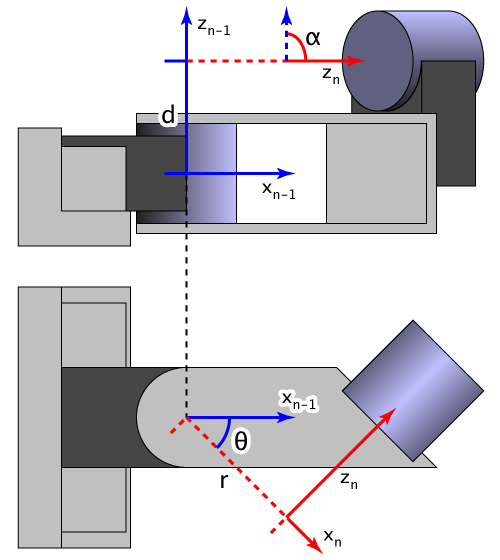
\includegraphics[width=0.8\columnwidth]{./examples/pix/Sample_Denavit-Hartenberg_Diagram.png}

	\subsection{Inverse Kinematics}\label{sec:ik}
			The next step is to find the inverse kinematic (IK) solution for the right arm.
Inherently this problem has multiple solutions.
When solving the IK Pieper\cite{peiper1968kinematics} states that a closed-form solution does exist if:
\begin{itemize}
\item Three consecutive joints axes of the manipulator are parallel to one another
\end{itemize}

OR
\begin{itemize}
\item Three consecutive joints intercect at a single point
\end{itemize}

The kinematic structure in Fig~\ref{fig:hubo} and Fig~\ref{fig:IkFkCoordinate} shows that the Hubo2+ platform does have a three joints that intersect the same point in the shoulders and in the hips.
Thus a closed-form solution exists for both arms and both legs.

The transform $T_0^6$ in Equation~\ref{eq:t06} is needed to solve the IK problem for the shoulder.  
It is important to note that $T_0^6$ is in the form of

\begin{equation}\label{eq:T06}
T_0^6 = \left[ \begin{array}{cccc} 
\overline{x_6} & \overline{y_6} & \overline{z_6} & \overline{p_6} \\
0              & 0              & 0              & 1   
\end{array} \right]
\end{equation} 

Where $\overline{x_6}$, $\overline{y_6}$ and $\overline{z_6}$ are $[3x1]$ unit vectors along the principle axes of the end-effectors coordinate frame $i$, see Fig.~\ref{fig:IkFkCoordinate}.
Position vector $\overline{p_6}$ describes the hand about joint $A1$ (shoulder).
The arm can be vied in different frames.
If we look at the arm in reference to the end-effector's frame.
The reverse transform is defined as $(T_0^6)`$


\begin{equation}
(T_0^6)' = T_6^0 = (T_0^6)^{-1} = \left[ \begin{array}{cccc} 
\overline{x_6} & \overline{y_6} & \overline{z_6} & \overline{p_6} \\
0              & 0              & 0              & 1   
\end{array} \right]^{-1}
\end{equation} 

The following method is based on the work done by our partner Park et. al.\cite{5649842}.
The general link translation matrix $T_{i-1}^i$ relates the $i^{th}$ coordinate frame to the $(i-1)^{th}$ coordinate frame.  
In addition we can extend Equation~\ref{eq:T06} to

\begin{equation}\label{eq:06invIK}
T_0^6 = \left[ \begin{array}{cccc} 
\overline{x_6} & \overline{y_6} & \overline{z_6} & \overline{p_6} \\
0              & 0              & 0              & 1   
\end{array} \right] = \left[ \begin{array}{cccc} 
\overline{n} & \overline{s} & \overline{a} & \overline{p} \\
0            & 0            & 0            & 1   
\end{array} \right]
\end{equation} 

Where $[\overline{n}, \overline{s}, \overline{a}, \overline{p}]$ represents the normal vector, the sliding vector, the approach vector and the position vector of the end effector respectively\cite{fu1987robotics}.  We can now state that

\begin{equation}
(T_0^6)' = T_6^0 = (T_0^6)^{-1} = \left[ \begin{array}{cccc} 
\overline{x_6} & \overline{y_6} & \overline{z_6} & \overline{p_6} \\
0              & 0              & 0              & 1   
\end{array} \right]^{-1}= \left[ \begin{array}{cccc} 
\overline{n}' & \overline{s}' & \overline{a}' & \overline{p}' \\
0             & 0             & 0             & 1   
\end{array} \right]
\end{equation} 

We can now use the reverse method to solve for the joint angles as in \cite{fu1987robotics} and derived in the tech report\cite{gtechIK2}.
The first three lower joint angles of $A_4$, $A_5$ and $A_6$ are solved for.
Subsequently the upper joint angles of $A_1$, $A_2$ and $A_3$ are solved.

Using inverse transform methods\cite{4046335} we can modify Equation~\ref{eq:t06} to

\begin{equation}\label{eq:t06IK}
T_6^0 = (T_0^6)^{-1} = \prod_{i=6}^{1} T_{i}^{i-1} = T_{6}^{5}T_{5}^{4}T_{4}^{3}T_{3}^{2}T_{2}^{1}T_{1}^{0}
\end{equation}

Then we equate Equation~\ref{eq:06invIK} to Equation~\ref{eq:t06IK} 

\begin{equation}
T_{6}^{5}T_{5}^{4}T_{4}^{3}T_{3}^{2}T_{2}^{1}T_{1}^{0} = \left[ \begin{array}{cccc} 
\overline{n}' & \overline{s}' & \overline{a}' & \overline{p}' \\
0             & 0             & 0             & 1   
\end{array} \right]
\end{equation}

Then move $T_6^5$ to the other side of the equation


\begin{equation}\label{eq:preG}
T_{5}^{4}T_{4}^{3}T_{3}^{2}T_{2}^{1}T_{1}^{0} = T_{5}^{6}\left[ \begin{array}{cccc} 
\overline{n}' & \overline{s}' & \overline{a}' & \overline{p}' \\
0             & 0             & 0             & 1   
\end{array} \right]
\end{equation}

For simplicity we will represent Equation~\ref{eq:preG} as $G_L$ and $G_R$ standing for \textit{right} and \textit{left} side.

\begin{equation}
G_L = T_{5}^{6}\left[ \begin{array}{cccc} 
\overline{n}' & \overline{s}' & \overline{a}' & \overline{p}' \\
0             & 0             & 0             & 1   
\end{array} \right]
\end{equation}



\begin{equation}
G_R = T_{5}^{4}T_{4}^{3}T_{3}^{2}T_{2}^{1}T_{1}^{0} 
\end{equation}


Expanding gives us

\begin{equation}
G_L = \left[ \begin{array}{cccc} 
g_{11} & g_{12} & g_{13} & cos(\theta_6)(p_x'+l_{A_4})-sin(\theta_6)p_y' \\
g_{21} & g_{22} & g_{23} & sin(\theta_6)(p_x'+l_{A_4})-cos(\theta_6)p_y' \\
g_{31} & g_{32} & g_{33} & p_z'                                         \\
0      & 0      & 0      & 1   
\end{array} \right]
\end{equation}

and

\begin{equation}
G_R = \left[ \begin{array}{cccc} 
g_{11} & g_{12} & g_{13} & sin(\theta_4)cos(\theta_5)l_{A_2} \\
g_{21} & g_{22} & g_{23} & -cos(\theta_6)l_{A_2}-l_{A3}       \\
g_{31} & g_{32} & g_{33} & sin(\theta_4)sin(\theta_5)l_{A_2}  \\
0      & 0      & 0      & 1   
\end{array} \right]
\end{equation}

We can then equate elements $(1,4)$, $(2,4)$ and $(3,4)$ of $G_L$ and $G_R$. 
This gives us

\begin{equation}\label{eq:thetaSolve11}
cos(\theta_6)(p_x'+l_{A_4})-sin(\theta_6)p_y' = sin(\theta_4)cos(\theta_5)l_{A_2}
\end{equation}

\begin{equation}\label{eq:thetaSolve12}
sin(\theta_6)(p_x'+l_{A_4})-cos(\theta_6)p_y' = -cos(\theta_6)l_{A_2}-l_{A3}
\end{equation}

\begin{equation}\label{eq:thetaSolve13}
p_z' = sin(\theta_4)sin(\theta_5)l_{A_2}
\end{equation}

Based on the desired task space location we let

\begin{equation}\label{eq:thetaSolve21}
p_x' + l_{A_4} = r \cdot cos(\phi)
\end{equation}

and

\begin{equation}\label{eq:thetaSolve22}
p_y' = r \cdot sin(\phi)
\end{equation}

where 

\begin{equation}\label{eq:thetaSolve31}
r = sqrt{(p_x'+l_{A_4})^2 + (p_y')^2}
\end{equation}

and 

\begin{equation}\label{eq:thetaSolve32}
\phi = atan2(p_y',p_x'+l_{A_4})
\end{equation}

\textbf{Note:} $atan2()$ represents the the $atan$ method that gathers the information of the signs of the inputs in order to put the returned value in the appropriate quadrant.

Combining Equation (\ref{eq:thetaSolve11}), (\ref{eq:thetaSolve12}) and (\ref{eq:thetaSolve13}) with Equation (\ref{eq:thetaSolve21}) and (\ref{eq:thetaSolve22}) we get

\begin{equation}\label{eq:thetaSolve41}
r \cdot cos(\theta_6+\phi) = sin(\theta_4)cos(\theta_5)l_{A_2}
\end{equation}

\begin{equation}\label{eq:thetaSolve42}
r \cdot sin(\theta_6+\phi) = -cos(\theta_4)l_{A_2}-l_{A_3}
\end{equation}

\begin{equation}\label{eq:thetaSolve43}
p_z' = sin(\theta_4)sin(\theta_5)l_{A_2}
\end{equation}


When we combine above with Equation (\ref{eq:thetaSolve31}) and (\ref{eq:thetaSolve32}) and obtain 


\begin{equation}
\theta_4 = atan2\left( \pm \sqrt{1-cos(\theta_4)^2} , cos(\theta_4)  \right)
\end{equation}

where

\begin{equation}
cos(\theta_4) = \frac{(p_x'+l_{A_4})^2  +  p_y'^2  +  p_z'^2  -  l_{A_2}^2  -  l_{A_3}^2}
                     {2l_{A_2}l_{A3}}
\end{equation}

Using Equation~\ref{eq:thetaSolve43} we can get $\theta_5$

\begin{equation}
\theta_5 = atan2(sin(\theta_5), \pm\sqrt{1-sin(\theta_5)^2})
\end{equation}

where

\begin{equation}
sin(\theta_5) = \frac{p_z'}
                     {sin(\theta_4)l_{A_2}}
\end{equation}


We can then solve for $\theta_6$ by dividing Equation~\ref{eq:thetaSolve42} by Equation~\ref{eq:thetaSolve41}.



\begin{equation}
\frac{r \cdot sin(\theta_6+\phi)}
     {r \cdot cos(\theta_6+\phi)} = tan(\theta_6+\phi) = \frac{-cos(\theta_4)l_{A_2}-l_{A_3}}
                                                              {sin(\theta_4)cos(\theta_5)l_{A_2}}
\end{equation}

\begin{equation}
\theta_6 = atan2(-(cos(\theta_4)l_{A_2}+l_{A_3}), sin(\theta_4)cos(\theta_5)l_{A_2}) - \phi
\end{equation}



\section{Verification: Door Opening}\label{sec:hubo-achVerification}
	Section~\ref{sec:timing}, \ref{sec:valve}, and \ref{sec:hubo-ach-kinimatics} verrified the functionality of Hubo-Ach under different circumstances.

\begin{figure}[thpb]
  \centering
      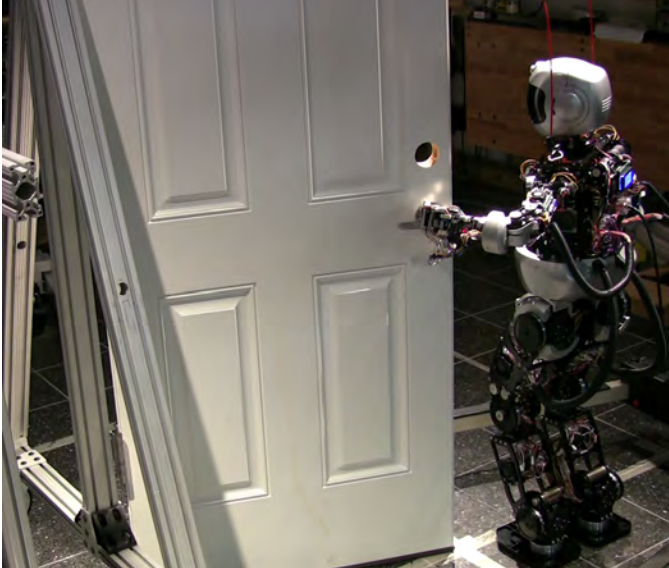
\includegraphics[width=0.69\columnwidth]{./pix/hubo-door.png}
\includegraphics[width=0.3\columnwidth]{./qrcode/qrcode-door.png}\\
http://danlofaro.com/phd/door/
      
\caption{Indipendent validation of Hubo-Ach via Zucker et. al.\cite{tepraDoor2013} work in\textit{Continuous Trajectory Optimization for Autonomous Humanoid Door Opening}.}
\label{fig:hubo-ach-door-open}
\end{figure}

Zucker et. al.\cite{tepraDoor2013} independently validates Hubo-Ach through their work in\textit{Continuous Trajectory Optimization for Autonomous Humanoid Door Opening}.
Fig.~\ref{fig:hubo-ach-door-open} shows Zucker's work




\section{Validation: Peer Survey on Hubo-Ach}
	This section shows the peer survey taken by users of Hubo-Ach.
	Thirteen independent users were surveyed.
	The overwhelming conclusion was that the system is useful, was the unifying algorithmic framework as advertised and helped with development.
	Out of a score from 0-10 on the question \textit{"Would you use Hubo-Ach again the the future when programming Hubo"} received an average of 9.23 (see Table~\ref{table:q6}.
	Table~\ref{table:q1}, \ref{table:q2}, \ref{table:q3}, \ref{table:q4}, \ref{table:q5}, \ref{table:q6}

	\begin{table}
\centering
\caption{Q1: Survey on the Unified Algorithmic Framework for Complex System and Humanoids, Hubo-Ach:}\label{table:q1}
Opinions about Hubo-Ach:\\
\small
10 = Agree, 0=Disagree\\
Sample Size = 13
\normalsize
%\begin{tabular}{l | l}
\begin{longtable}{|p{9cm} | p{4cm} | }
\hline
Question	&	Average Rating (0-10)	\\	\hline
\hline
\hline
It is easy to use Hubo-Ach													& 8.77\\
\hline
It is easy to integrate Hubo-Ach into your existing controllers/systems 							& 7.69\\
\hline
Hubo-Ach makes it conducive for you to use pre-existing tools (such as ROS, OpenRAVE, DART, Custom Software, etc.)		& 8.31\\
\hline
The multi-process methodology of Hubo-Ach makes it easy for you to implement your controllers in any language you desire.	& 8.85\\
\hline
Hubo-Ach is easier to use then other high DOF real-time robot software you have used in the past				& 8.62\\
\hline

\end{longtable}

\end{table}

	\begin{table}
\centering
\caption{Q2: Survey on the Unified Algorithmic Framework for Complex System and Humanoids, Hubo-Ach:}\label{table:q2}
Hubo-Ach and your controller implementations:\\
\small
10 = Agree, 0=Disagree\\
Sample Size = 13\\
\normalsize
%\begin{tabular}{l | l}
\begin{longtable}{|p{9cm} | p{3cm} | }
\hline
Question	&	Average Rating (0-10)	\\	\hline
\hline
\hline
You successfully integrated Hubo-Ach into your existing controllers/systems							& 9.15\\
\hline
The latency in Hubo-Ach does not have a noticeable effect on your controllers 							& 9.38\\
\hline
The sampling frequency does not have a noticeable effect of your controllers							& 9.15\\
\hline


\end{longtable}
\end{table}


	\begin{table}
\centering
\caption{Q3: Survey on the Unified Algorithmic Framework for Complex System and Humanoids, Hubo-Ach:}\label{table:q3}
What programming languages do you interface with Hubo-Ach:\\
\small
10 = Often, 0=Never\\
Sample Size = 13\\
\normalsize
%\begin{tabular}{l | l}
\begin{longtable}{|p{9cm} | p{3cm} | }
\hline
Question	&	Average Rating (0-10)	\\	\hline
\hline
\hline
C/C++		& 	9.3 \\
\hline
Python		&	7.69\\
\hline
MATLAB		&	3.15 \\
\hline		
Other		&	1.92 \\
\hline


\end{longtable}
\end{table}

	\begin{table}
\centering
\caption{Q4: Survey on the Unified Algorithmic Framework for Complex System and Humanoids, Hubo-Ach:}\label{table:q4}
What simulators do you use in conjunction with Hubo-Ach:\\
\small
10 = Often, 0=Never\\
Sample Size = 13\\
\normalsize
%\begin{tabular}{l | l}
\begin{longtable}{|p{9cm} | p{3cm} | }
\hline
Question	&	Average Rating (0-10)	\\	\hline
\hline
\hline
DART		& 	3.23 \\
\hline
OpenHubo	&	7.54\\
\hline
RobotSim	&	2.54 \\
\hline		
Other		&	3.92 \\
\hline


\end{longtable}
\end{table}

	\begin{table}
\centering
\caption{Q5: Survey on the Unified Algorithmic Framework for Complex System and Humanoids, Hubo-Ach:}\label{table:q5}
Choice of Hubo Software: Given the choice, how likely is it that you would use the following software platforms to implemented your controllers on Hubo.:\\
\small
10 = Very Likely, 0=Unlikely\\
Sample Size = 13\\
\normalsize
%\begin{tabular}{l | l}
\begin{longtable}{|p{9cm} | p{3cm} | }
\hline
Question		&	Average Rating (0-10)	\\	\hline
\hline
\hline
ACES/Conductor		& 	2.69 \\
\hline
Hubo-Ach		&	9.51 \\
\hline
Maestro			& 	5.42 \\
\hline
RAINBOW (Windows)	&	3.46 \\
\hline
RAINBOW (Xenomai)	&	4.00 \\
\hline


\end{longtable}
\end{table}


	\begin{table}
\centering
\caption{Q6: Survey on the Unified Algorithmic Framework for Complex System and Humanoids, Hubo-Ach:}\label{table:q6}
Effects of Hubo-Ach:\\
\small
10 = Agree, 0=Disagree\\
Sample Size = 13\\
\normalsize
%\begin{tabular}{l | l}
\begin{longtable}{|p{9cm} | p{3cm} | }
\hline
Question		&	Average Rating (0-10)	\\	\hline
\hline
\hline
Without Hubo-Ach physically implementing your controllers on Hubo would have been much more difficult	& 	9.00 \\
\hline
Hubo-Ach was a key component is quickly implementing your controllers on the physical Hubo		&	9.15 \\
\hline
You would use Hubo-Ach again in the future when programming Hubo					& 	9.23 \\
\hline

\end{longtable}
\end{table}



In conclusion Hubo-Ach is validated as being a useful \textit{unified algorithmic framework for complex systems and humanoid robots} by peers.
Shown to have consistent system performance in Section~\ref{sec:timing}.
It is verified via implementation of full body kinematic examples in Section~\ref{sec:valve} and \ref{sec:6dofik}.








